\documentclass{article}
\usepackage[utf8]{inputenc}
\usepackage[italian]{babel}
\usepackage{amsmath}
\usepackage{amssymb}
\usepackage{siunitx}
\usepackage{tabularray}
\usepackage{graphicx}
\usepackage{float}
% \usepackage{minted}
\usepackage[bottom]{footmisc}
\usepackage[justification=centering]{caption}    % for \caption*{}
\usepackage[labelformat=simple, justification=centering]{subfig}
\usepackage[page]{appendix}
\renewcommand{\thesubfigure}{}
\newcommand*{\diam}{\varnothing}
\newcommand*{\best}[1]{{#1}_\text{best}}
\newcommand*{\bestp}[1]{{\left(#1\right)}_\text{best}}
\newcommand*{\pbest}[1]{\left({#1}_\text{best}\right)}
\newcommand*{\pbestp}[1]{\left({\left(#1\right)}_\text{best}\right)}
\newcommand*{\errrel}[1]{\frac{\delta #1}{{#1}_\text{best}}}
\title{
  Laboratorio di Fisica 1\\
  R9: Misura della viscosità della glicerina
}
\author{Gruppo 15: Bergamaschi Riccardo, Graiani Elia, Moglia Simone}
\date{16/04/2024 – 23/04/2024}
\makeindex
\begin{document}

\maketitle

\begin{abstract}
  Il gruppo di lavoro ha misurato la concentrazione e il coefficiente di
  viscosità di una soluzione acquosa di glicerina, studiando il moto di
  caduta di svariate sferette all'interno di essa.
\end{abstract}

\setcounter{section}{-1}
\section{Materiali e strumenti di misura utilizzati}
\begin{center}
  \begin{tblr}{
    width=\textwidth,
    colspec={ X[2,m,j]X[1,m,c]X[1,m,c]X[1,m,c] },
    vlines,
  }
    \hline
    \textbf{Strumento di misura} & \textbf{Soglia} & \textbf{Portata} & \textbf{Sensibilità} \\
    \hline
    Cronometro & $\qty{0.033}{s}$ & N./A. & $\qty{0.033}{s}$ \\
    \hline[dashed]
    Micrometro ad asta filettata & $\qty{0.01}{mm}$ & $\qty{25.00}{mm}$ & $\qty{0.01}{mm}$ \\
    \hline[dashed]
    Metro a nastro & $\qty{0.1}{cm}$ & $\qty{300.0}{cm}$ & $\qty{0.1}{cm}$ \\
    \hline[dashed]
    Bilancia di precisione & $\qty{0.01}{g}$ & $\qty{6200.00}{g}$ & $\qty{0.01}{g}$ \\
    \hline[dashed]
    Termometro ambientale & ? & ? & $\qty{0.2}{\degree C}$ \\
    \hline
  \end{tblr}
  \begin{tblr}{
    width=\textwidth,
    colspec={ X[m,j]X[3,m,j] },
    vlines,
  }
    \hline
    \textbf{Altro} & \textbf{Descrizione/Note} \\
    \hline
    Telecamera & Utilizzata per acquisire fotogrammi del sistema
      a intervalli regolari. \\
    \hline[dashed]
    Cilindro finito & {
      Utilizzato per contenere la glicerina. Su di esso sono indicati,
      con nastro adesivo nero, due traguardi.
    } \\
    \hline[dashed]
    Sferette & {
      %TODO:trovare un nome alternativo per le sferette
      Distribuibili in tre classi (“piccole”, “medie” o “grandi”)
      sulla base di diametro e massa.
    } \\
    \hline[dashed]
    Pinzetta & Per maneggiare le sferette. \\
    \hline[dashed]
    Tappo del cilindro & {
      Per contenere le sferette durante la misurazione della massa.
    } \\
    \hline
  \end{tblr}
\end{center}

\pagebreak
\section{Esperienza e procedimento di misura}

\begin{enumerate}
  \item Misuriamo la temperatura ambiente $T_\text{amb}$ per assicurarci
    che non sia cambiata significativamente dall'acquisizione precedente.
  \item Misuriamo la distanza tra i due traguardi $L = (18.0\pm0.1)\,\unit{cm}$
    con il metro a nastro.
  \item Per ogni classe $k$ di sferette:
  \begin{enumerate}
    \item
      Contiamo le sferette della classe $k$ (indicheremo questo numero
      con $N_k$).
    \item
      Misuriamo la massa media\footnote{
        Abbiamo misurato direttamente la massa totale $m_k^\text{tot}$
        mediante la bilancia di precisione, per poi calcolare
        $\overline{m}_k = \frac{1}{N_k} m_k^\text{tot}$,
        assumendo tutte le sferette di ugual massa.
      } $\overline{m}_k$ e il raggio medio\footnote{
        Essendo le sferette essenzialmente indistinguibili, abbiamo
        misurato direttamente, per ogni classe $k$, tre diametri con
        il micrometro ad asta filettata, per poi calcolarne la media
        $\overline{d}_k$ e ottenere il raggio con la semplice
        $\overline{r}_k = \frac{1}{2} \overline{d}_k$.
        Il gruppo di lavoro ritiene che si tratti di una buona stima
        per il raggio medio di tutte le sferette, anche considerato
        il fatto che i tre valori, in tutte le misurazioni, erano
        compatibili fra loro.
      } $\overline{r}_k$ di tutte e $N_k$ le sferette.
    \item Per ogni sferetta $i$:
    \begin{enumerate}
      \item
        Avviamo l'acquisizione del filmato sulla videocamera.
      \item
        Rilasciamo $i$ da ferma, poco sopra la superficie della soluzione,
        nel contenitore della glicerina, assicurandoci che la sua traiettoria
        non si avvicini alle pareti del recipiente\footnote{
          Quest'ultima richiesta sarà chiarita nella sezione 2.
        }.
      \item
        Al termine del moto della sferetta, interrompiamo la registrazione.
    \end{enumerate}
  \end{enumerate}
\end{enumerate}

L'esperienza è stata ripetuta completamente in due giornate differenti,
con $T_{\text{amb},1} = (24.6\pm0.2)\,\unit{\degree C}$
e $T_{\text{amb},2} = (19.4\pm0.2)\,\unit{\degree C}$.
Ciò si è rivelato molto utile per poter valutare la
coerenza dei risultati ottenuti, anche alla luce della
notevole differenza tra le due temperature.


\section{Analisi dei dati raccolti e conclusioni}
\emph{\textbf{Nota.}
Avendo valutato gli errori sulle grandezze misurate direttamente
come piccoli, casuali e indipendenti, per svolgere ogni calcolo
abbiamo utilizzato la tradizionale propagazione degli errori.
}

\subsection{Il modello fisico}

Scelta arbitrariamente una sferetta $i$ appartenente alla classe $k$,
fissiamo un sistema di riferimento cartesiano ortogonale, con asse
$z\parallel\vec{g}$ e origine nel punto in cui la sferetta viene rilasciata.
% TODO: L'origine va bene?

\vspace{2mm}
\emph{
  \textbf{Notazione.} Indicheremo con $\rho_\text{\emph{sf}}$ e
  $\rho_\text{\emph{sol}}$ le densità, rispettivamente, delle sferette
  e della soluzione e con $\eta$ la viscosità di quest'ultima.
}
\vspace{2mm}

Possiamo ora studiare la dinamica del corpo tra i due traguardi.
Per semplificare la discussione, assumeremo:
\begin{enumerate}
  \item Che il moto del centro di massa sia rettilineo uniforme con velocità
    $\vec{v}_i\parallel\vec{g}$;
  \item Che il moto avvenga in regime laminare
    (ovvero $\text{Re}=\frac{1}{\eta}\rho_\text{sol}\diam v_i \ll 1200$,
     dove $\diam$ è il diametro del recipiente);
  \item Che, rispetto alla sferetta, il recipiente possa essere
    considerato di dimensione indefinita: che si possano, cioè,
    trascurare gli effetti di bordo;
  \item Che il diametro $2r_i$ non superi, in ordine di grandezza,
    $10^{-3}\,\unit{m}$.
\end{enumerate}
Valuteremo più avanti, alla luce dei dati raccolti e dei risultati ottenuti,
se queste condizioni sono state verificate.

\vspace{2mm}

Le forze applicate alla sferetta sono la forza peso, la spinta di Archimede
e la forza di attrito viscoso $\vec{F}_\eta$.
Sotto le ipotesi (2.), (3.) e (4.), $\vec{F}_\eta$ può essere espressa come
$\vec{F}_\eta = -6\pi\eta r_i v_i\hat{z}$.

Allora, dalla prima legge di Newton:
\[
  \frac{4}{3}\pi g r_i^3 (\rho_\text{sf} - \rho_\text{sol}) \hat{z}
  -6\pi\eta r_i v_i\hat{z} = 0
\]
ovvero:
\[
  v_i = \frac{2g(\rho_\text{sf} - \rho_\text{sol})}{9\eta} r_i^2
\]
Per semplificare i calcoli, il gruppo di lavoro ha assunto tutte le sferette
della stessa classe essenzialmente indistinguibili. Sono stati perciò messi
in relazione i valori medi per ogni classe: \[
  \overline{v}_k = \frac{2g(\rho_\text{sf} - \rho_\text{sol})}{9\eta}
  \overline{r}_k^2
\]

\subsection{Misura della densità media di tutte le sferette}
Per calcolare $\rho_\text{sf}$, il gruppo di lavoro ha scelto di
effettuare una media ponderata delle densità medie delle tre classi:
\[
  \rho_\text{sf} = \frac{1}{\sum_k N_k} \sum_k \overline{\rho}_k N_k
    = \frac{1}{\sum_k N_k} \sum_k \frac{\overline{m}_k}{
      \frac{4}{3}\pi \overline{r}_k^3} N_k
    = \frac{3}{4\pi} \frac{1}{\sum_k N_k} \sum_k \frac{\overline{m}_k}{
      \overline{r}_k^3} N_k
  % \frac{
  %   \rho_\text{piccole} N_\text{piccole} +
  %   \rho_\text{medie} N_\text{medie} +
  %   \rho_\text{grandi} N_\text{grandi}}
  %   {N_\text{piccole} + N_\text{medie} + N_\text{grandi}}
\]
La densità media delle sferette è risultata essere,
in entrambi i giorni, $(7.713\pm0.045)\,\unit{kg \per dm^3}$.

\subsection{Misura e distribuzioni delle velocità}
Per determinare la velocità limite di ogni sferetta, il gruppo di
lavoro ha tracciato la quota di quest'ultima rispetto al secondo traguardo
in ogni fotogramma del relativo filmato.
Poiché ciascun fotogramma corrisponde a un istante
di tempo, è stato possibile ottenere così un grafico della quota in funzione
del tempo.

Il gruppo di lavoro ha poi eseguito una regressione lineare sui dati così
raccolti, per determinare la velocità media della relativa sferetta.

Riportiamo qui soltanto uno dei 131 grafici così ottenuti
(sferetta $1$, piccola, primo giorno):
\begin{figure}[H]
  \centering
  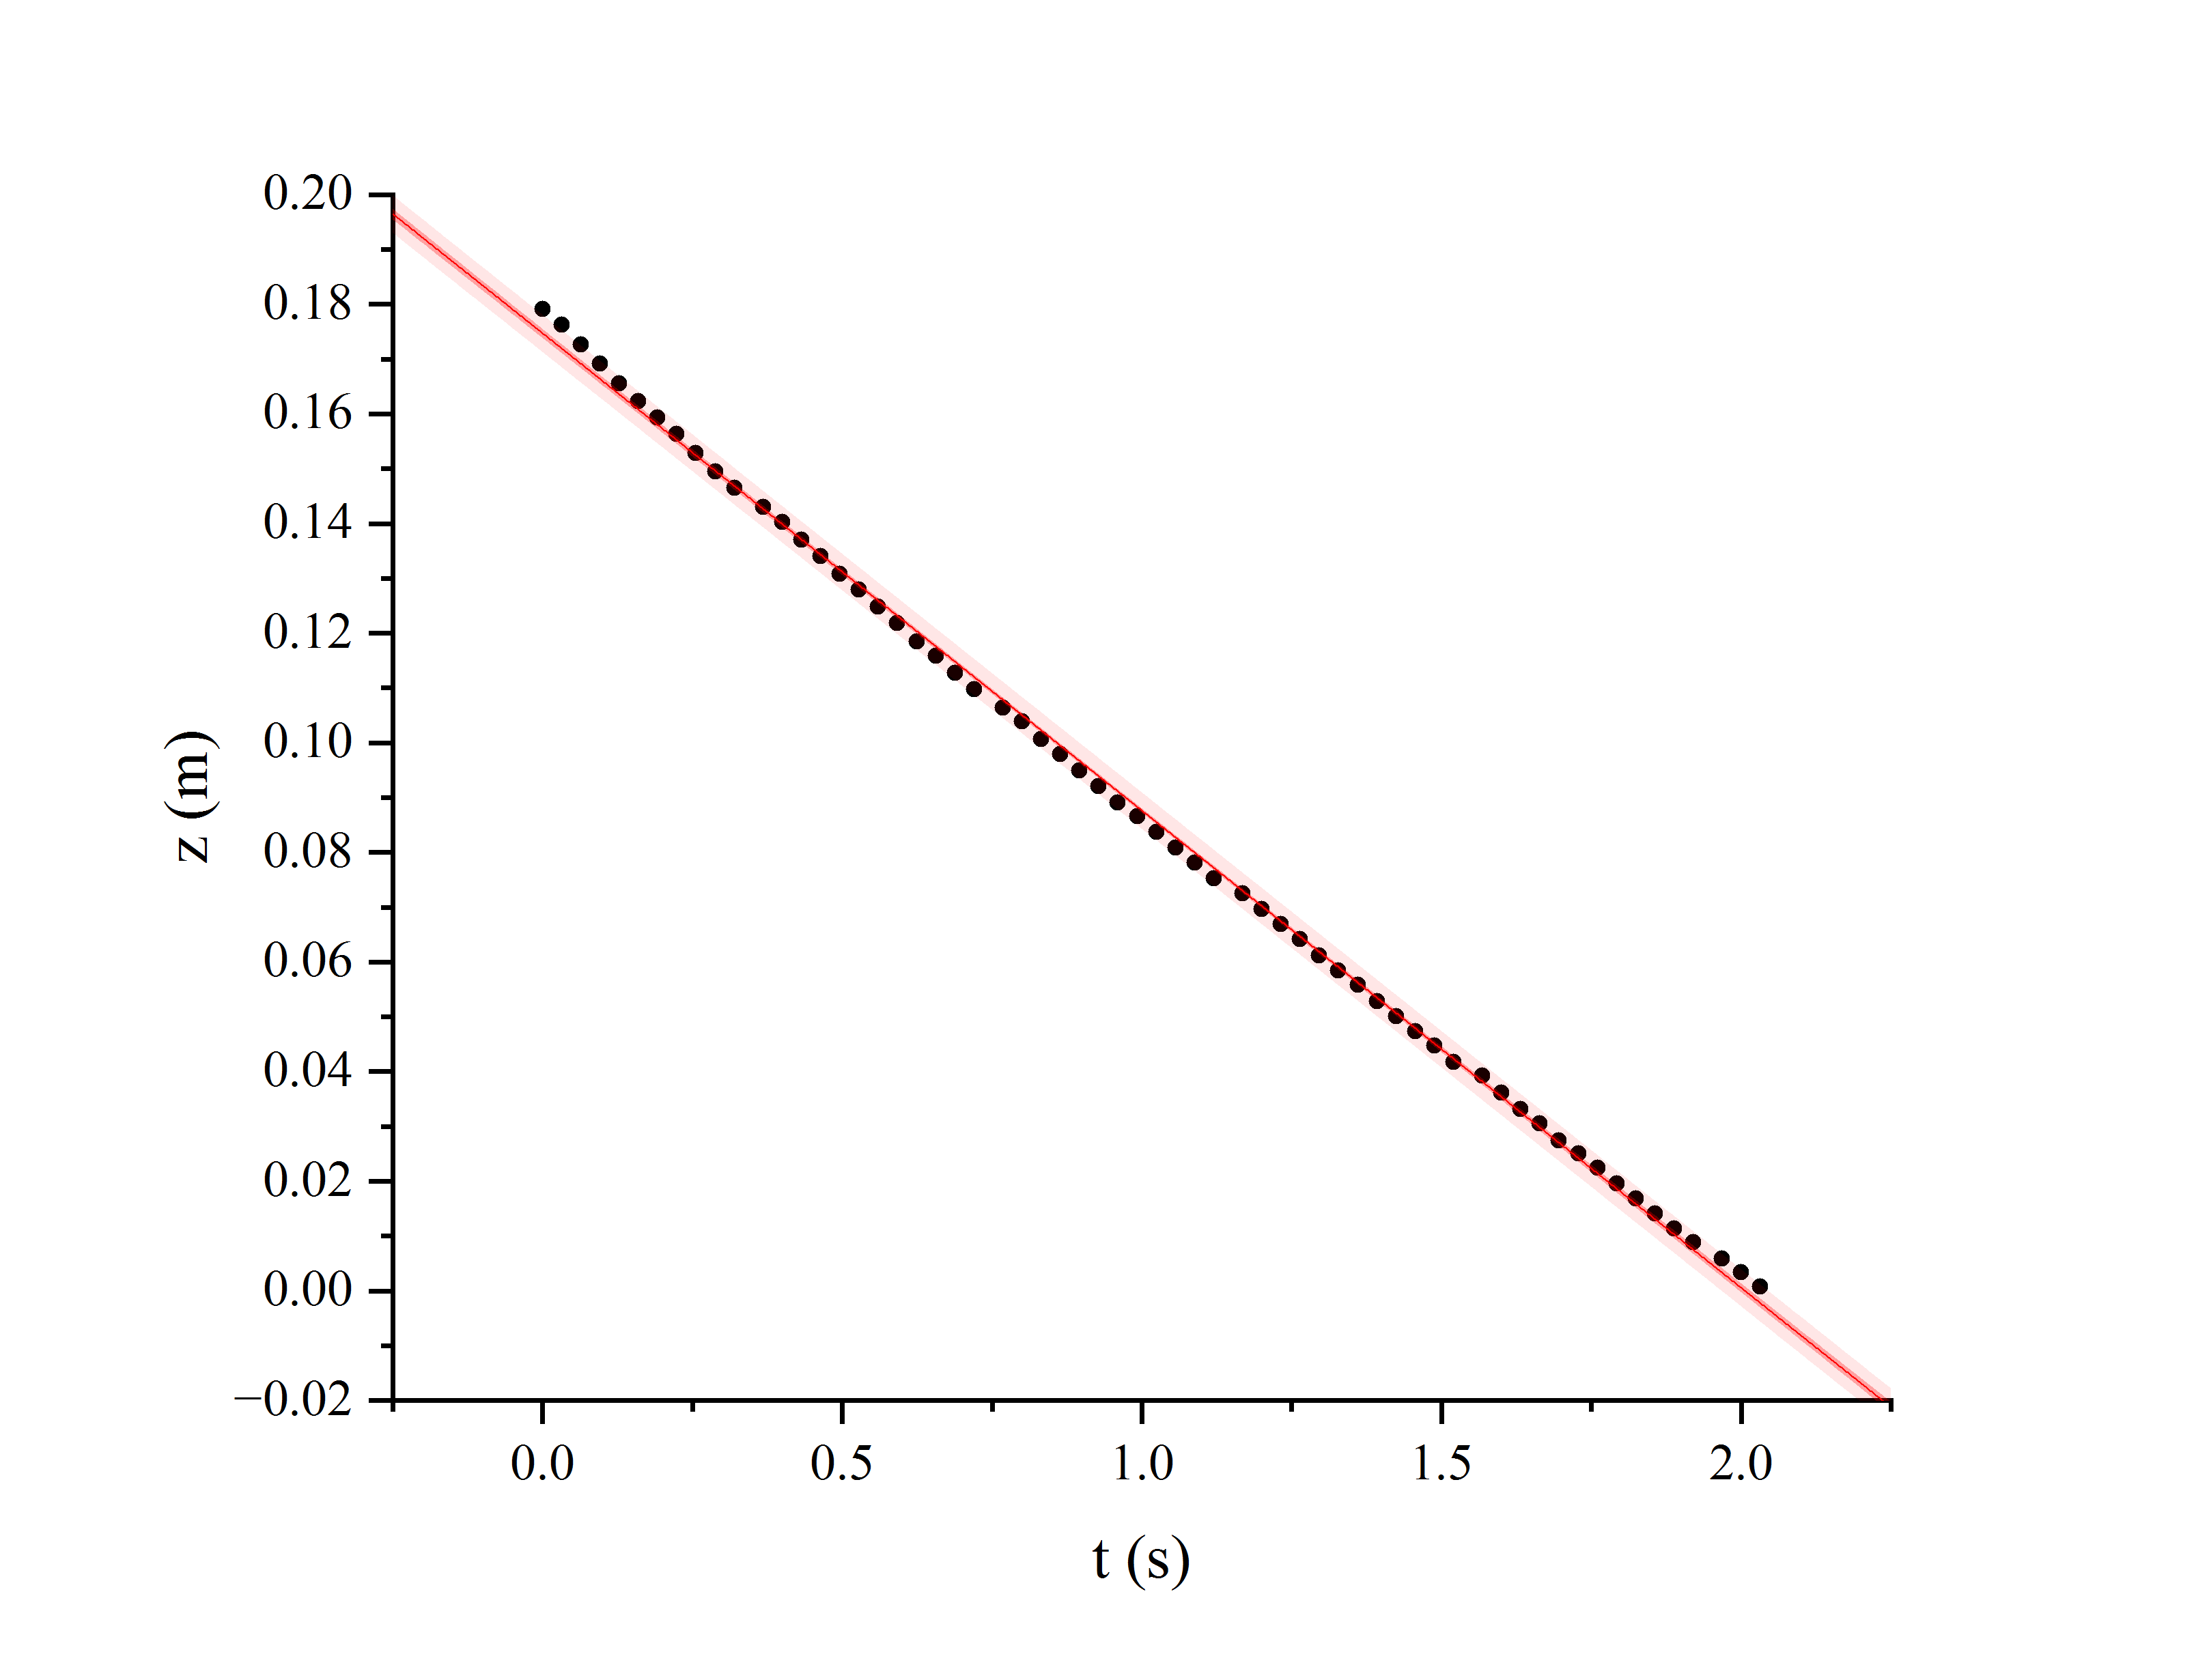
\includegraphics[trim={1.5cm 0.6cm 2cm 1cm},clip,width=\textwidth]{img/reg-p.png}
  \caption{\emph{
    In rosso la retta di regressione, in rosa la sua regione di incertezza.
  }}
\end{figure}

\pagebreak
Di seguito riportiamo le distribuzioni delle velocità per ogni classe
di sferette, di entrambi i giorni:
\vspace{-5mm}
\begin{center}
  \begin{figure}[H]
    % <v>^
    \centering
    \subfloat[][
      Primo giorno: Piccole ($N=12$)

      $\overline{v}=(8.738\pm0.016)\cdot10^{-2}\,\unit{m\per s}$
    ]{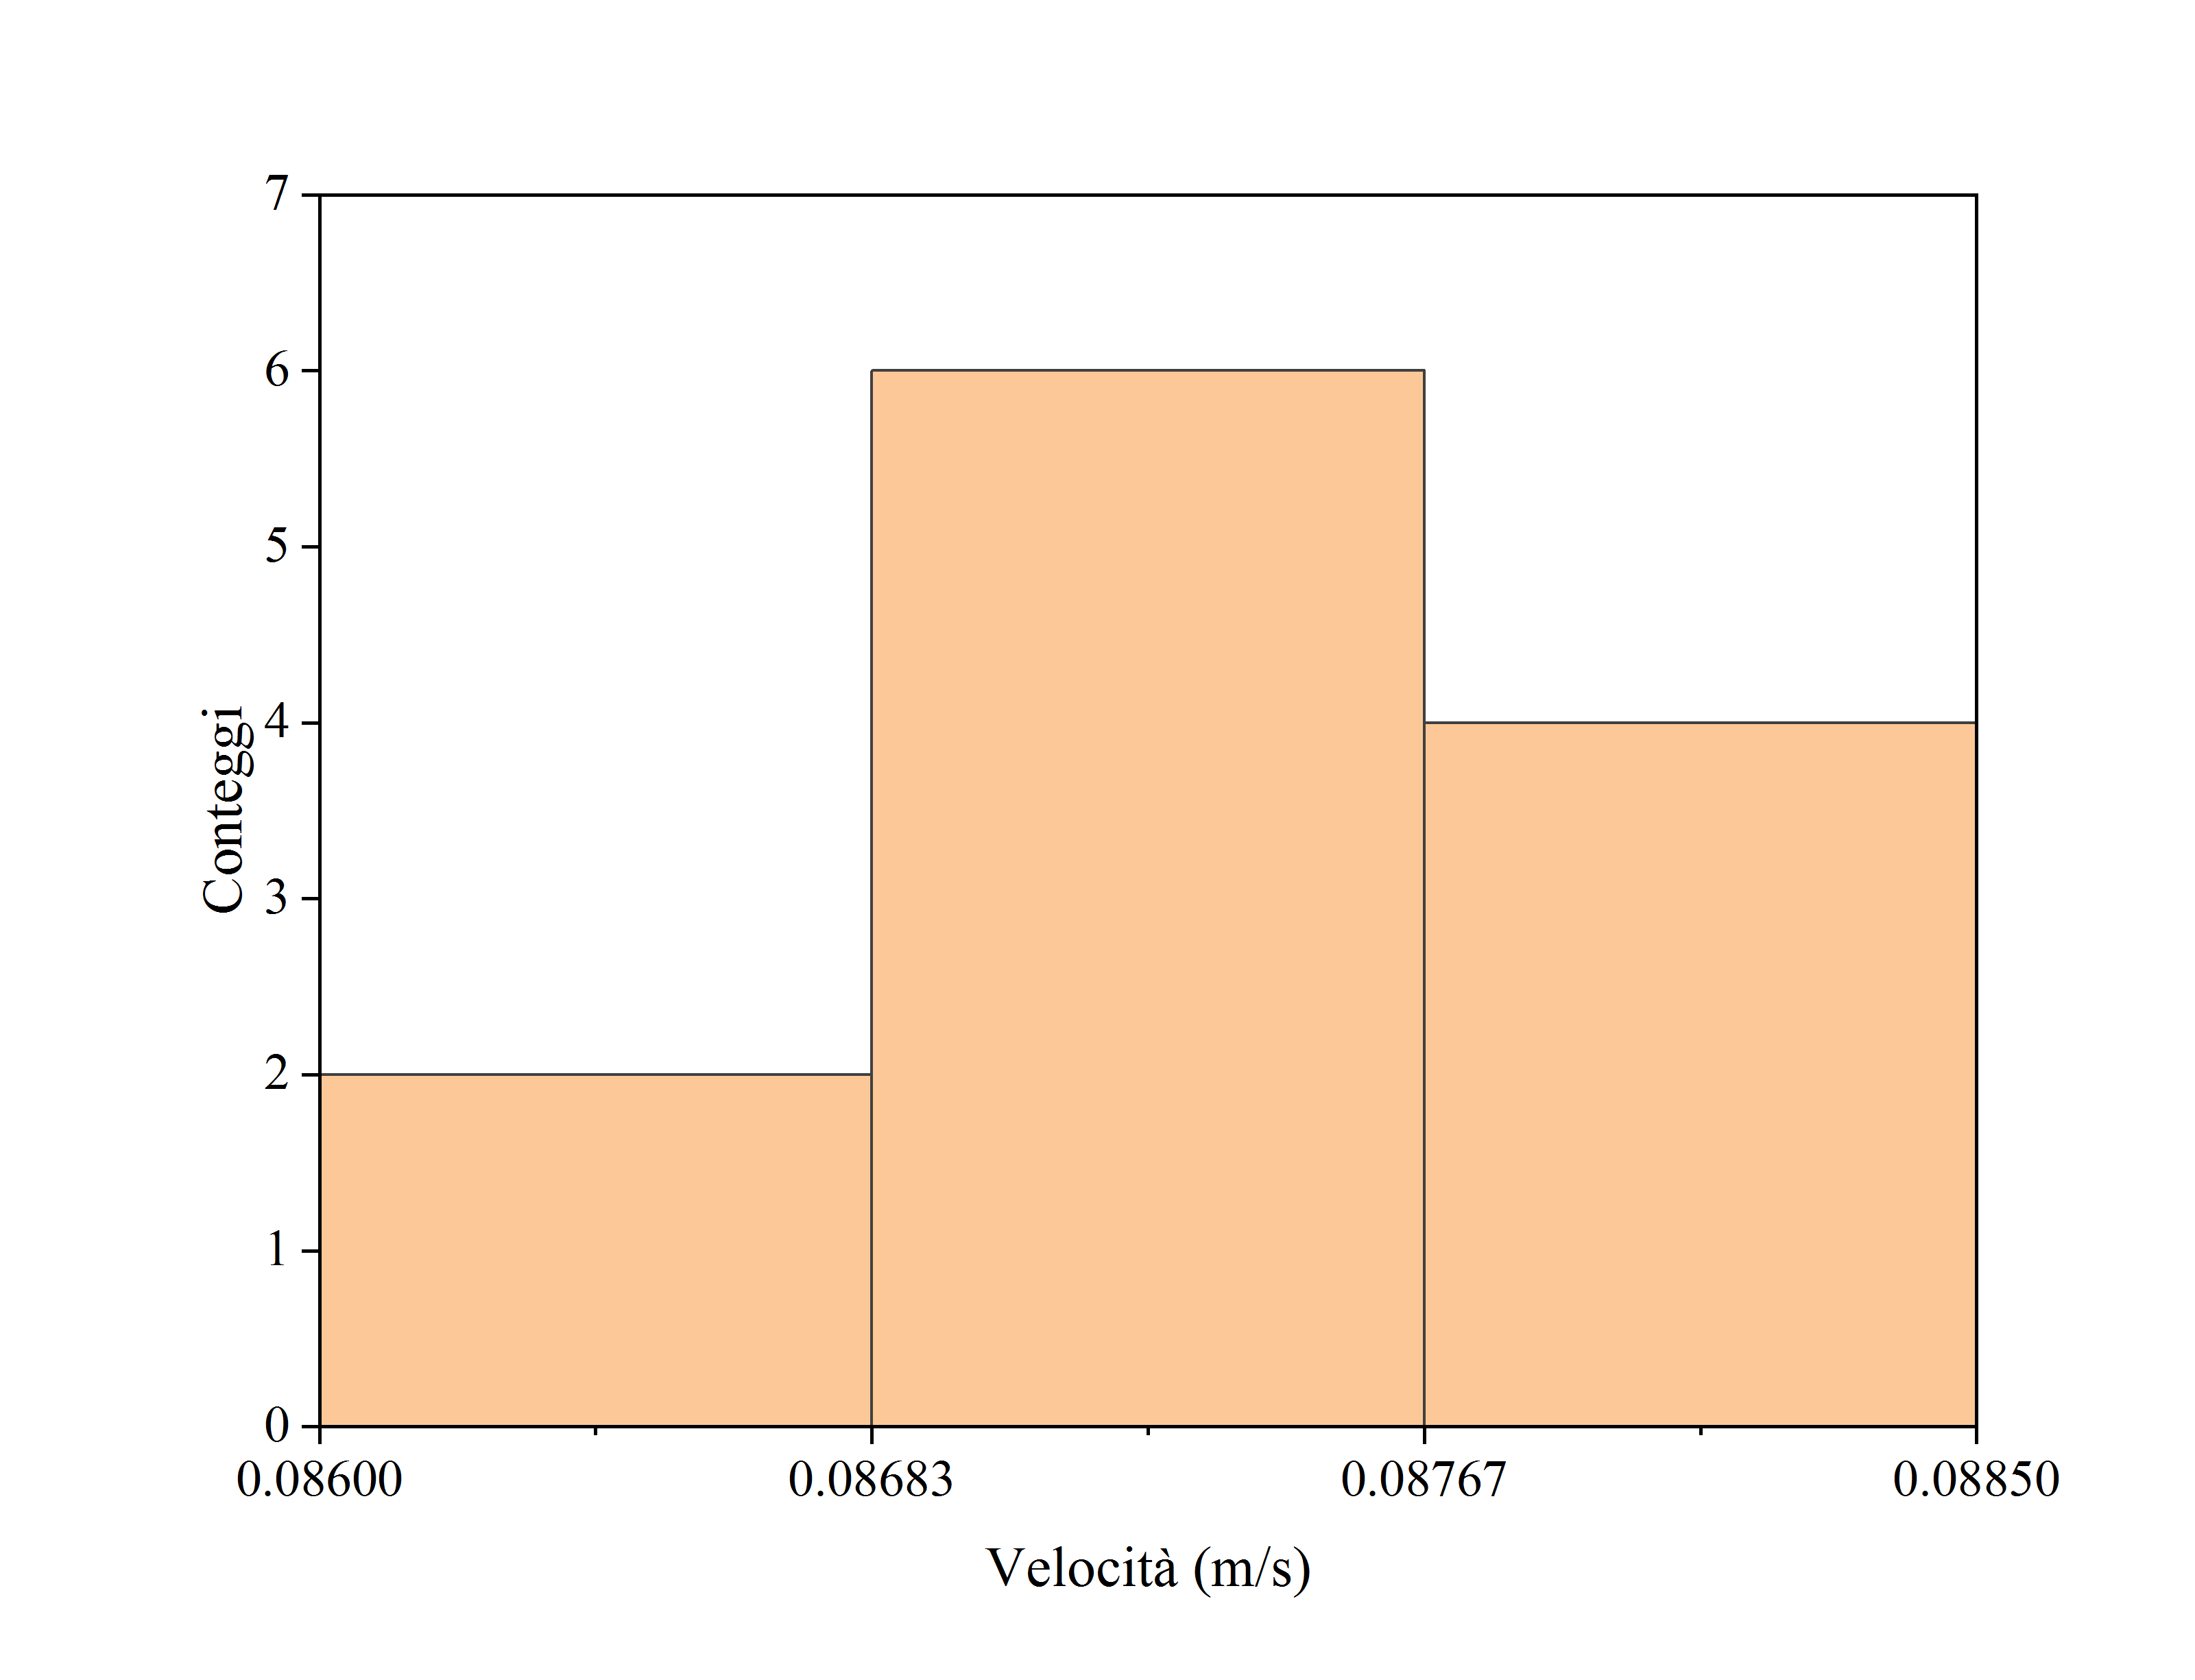
\includegraphics[trim={1cm 0.6cm 1cm 1cm},clip,width=.49\textwidth]{img/p1.png}}
    \hfil\subfloat[][
      Secondo giorno: Piccole ($N=13$)

      $\overline{v}=(5.65\pm0.02)\cdot10^{-2}\,\unit{m\per s}$
    ]{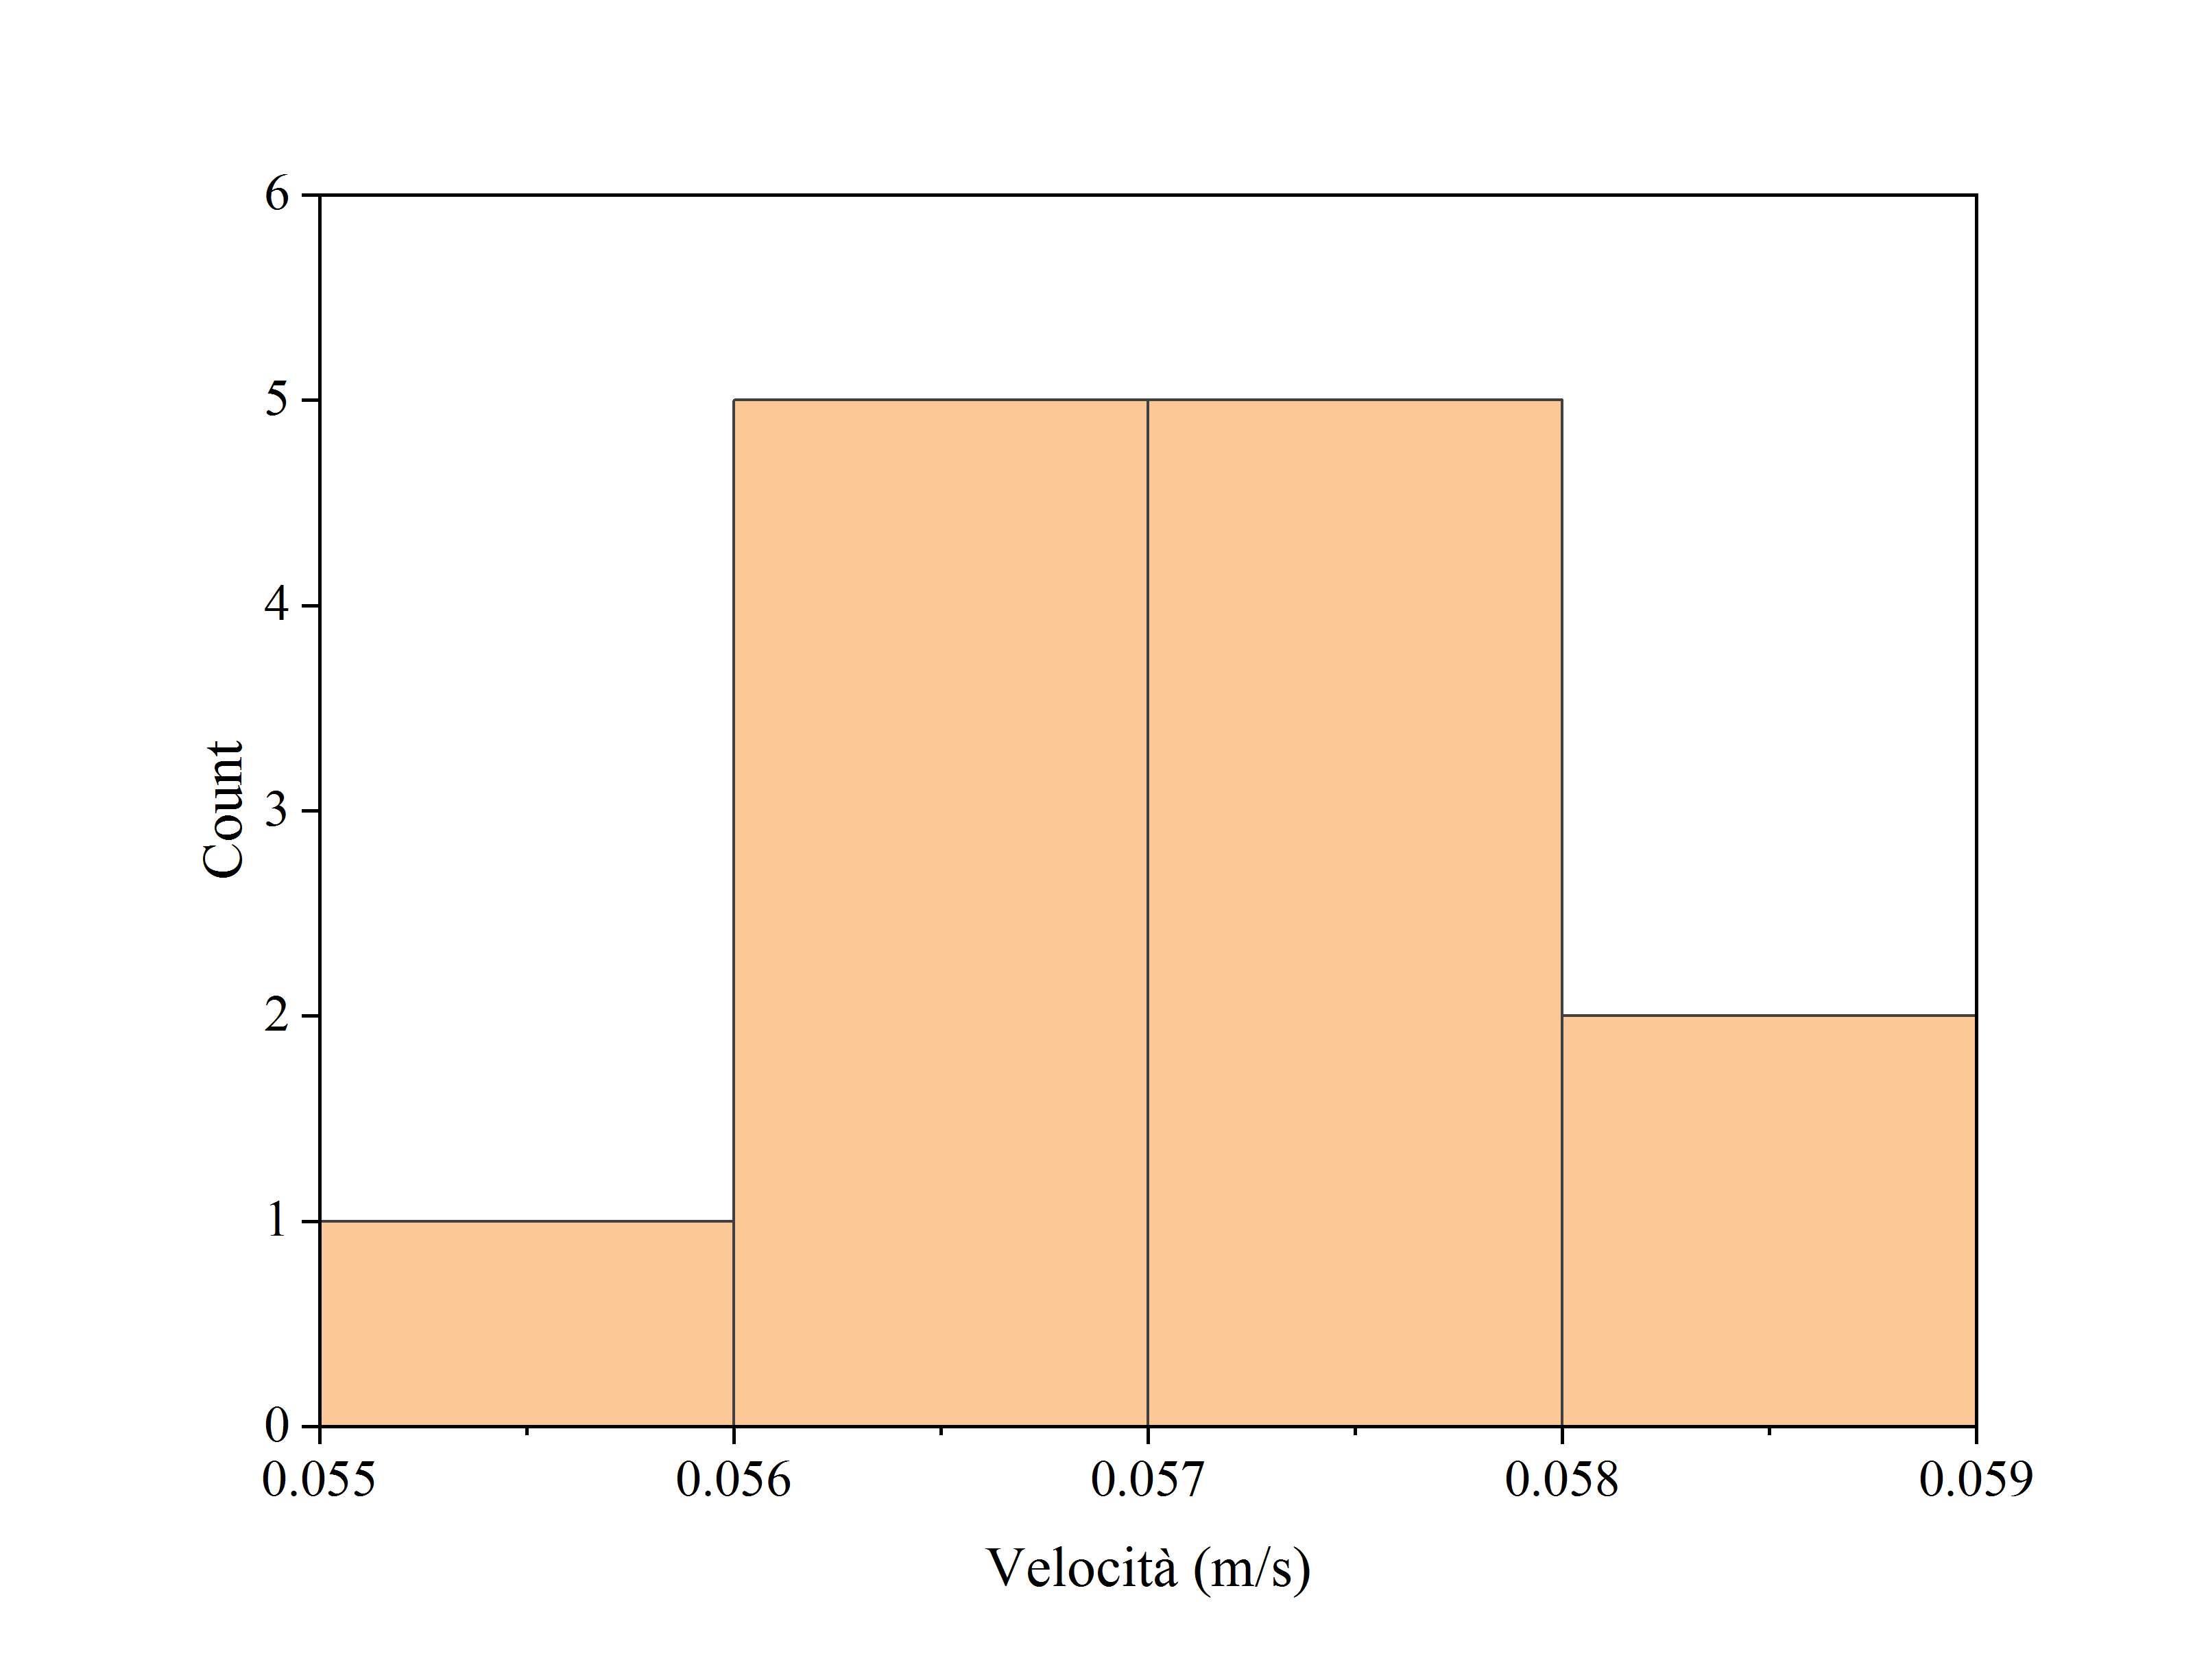
\includegraphics[trim={1cm 0.6cm 1cm 1cm},clip,width=.49\textwidth]{img/p2.png}}
    \hfil\subfloat[][
      Primo giorno: Medie ($N=23$)

      $\overline{v}=(12.97\pm0.03)\cdot10^{-2}\,\unit{m\per s}$
    ]{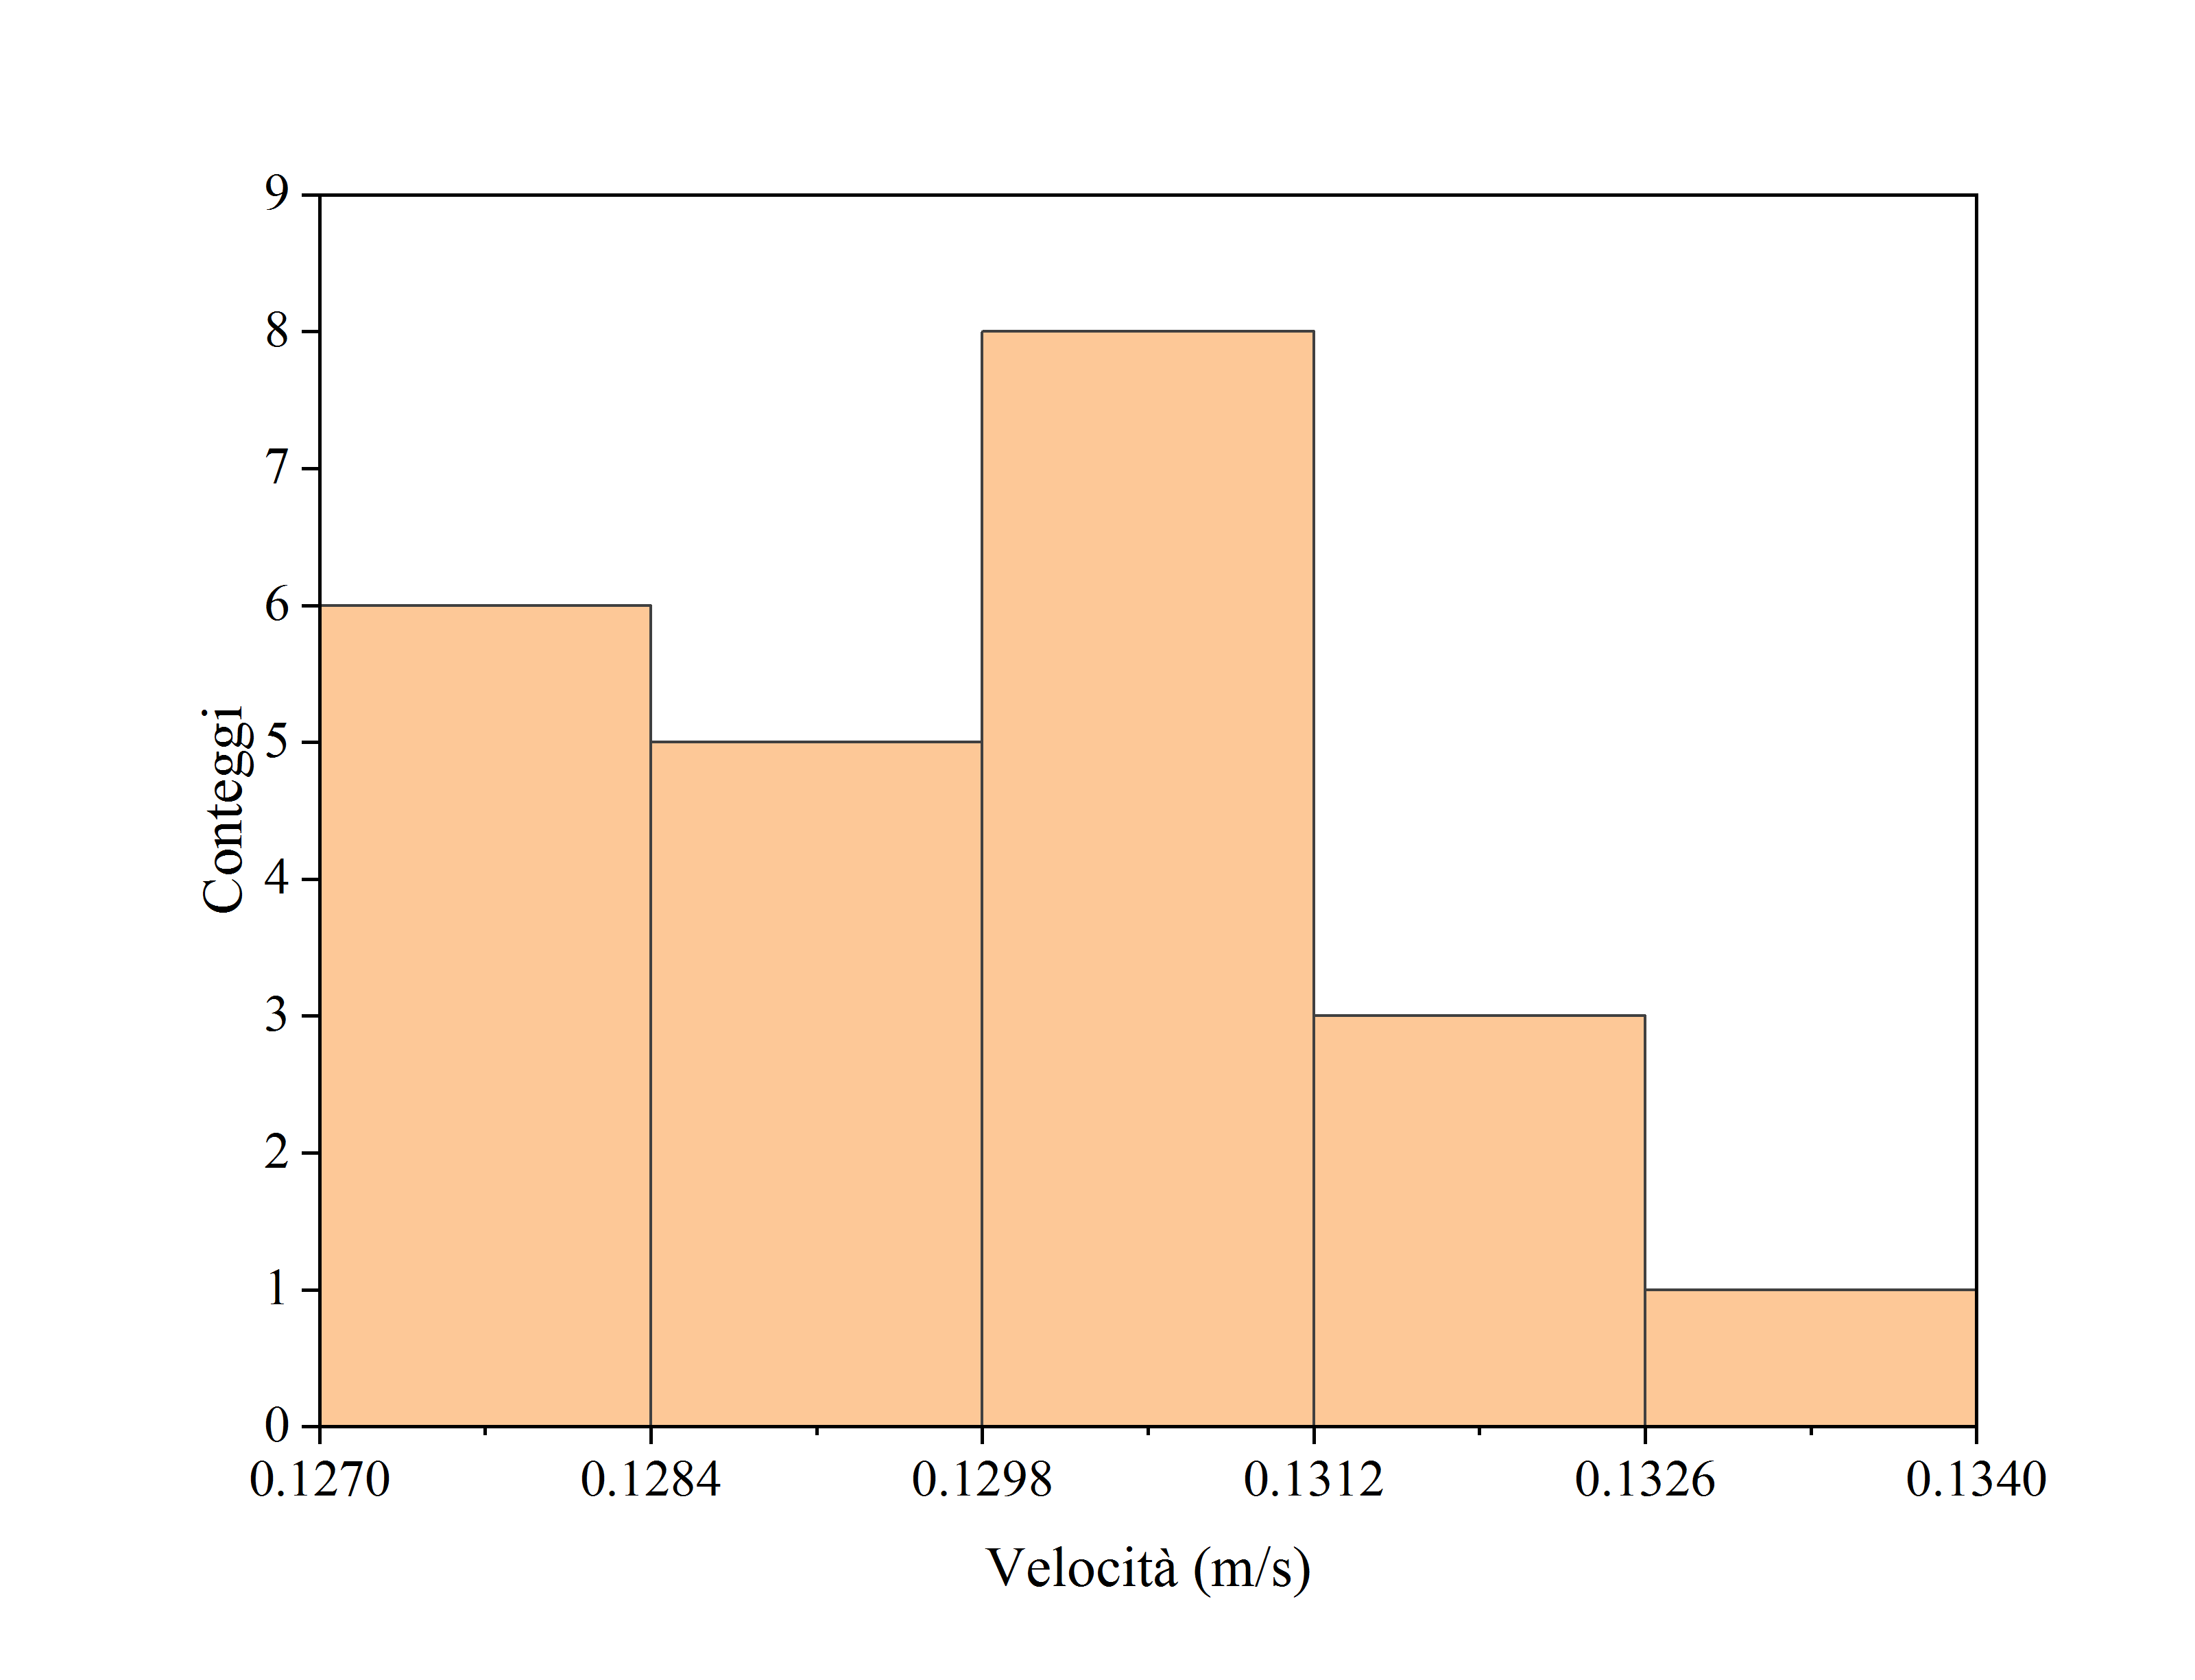
\includegraphics[trim={1cm 0.6cm 1cm 1cm},clip,width=.49\textwidth]{img/m1.png}}
    \hfil\subfloat[][
      Secondo giorno: Medie ($N=23$)

      $\overline{v}=(8.61\pm0.04)\cdot10^{-2}\,\unit{m\per s}$
    ]{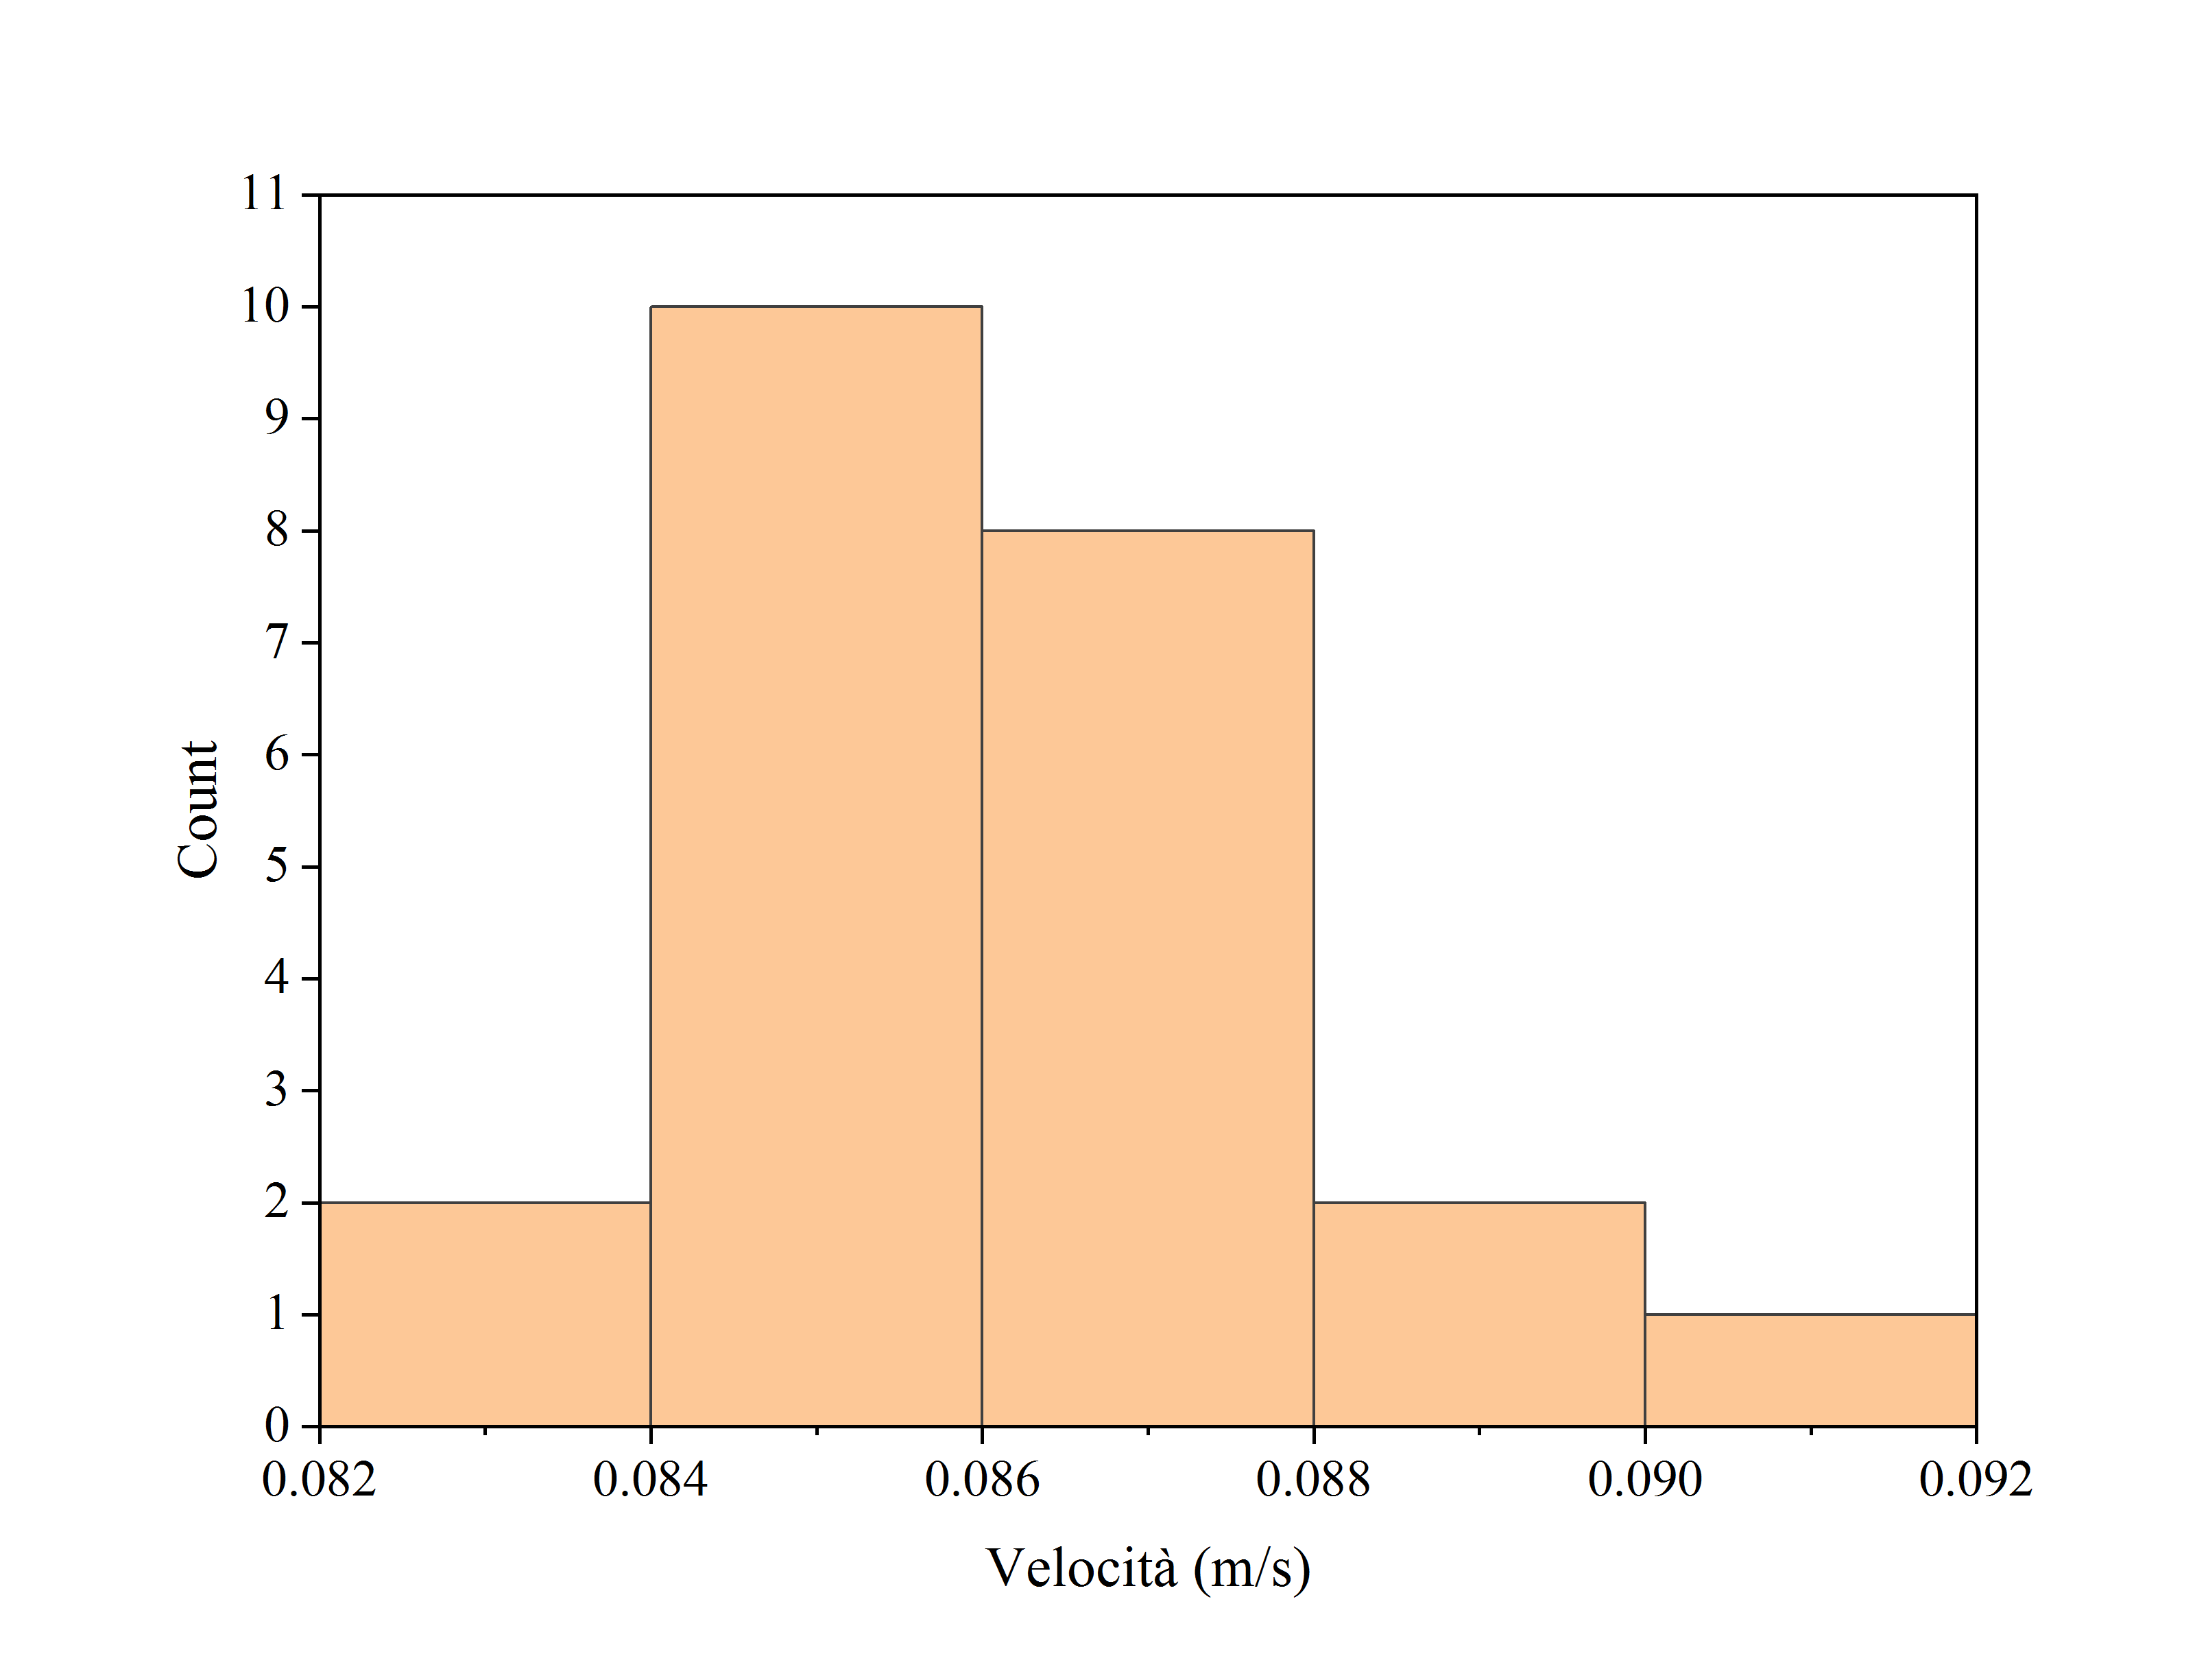
\includegraphics[trim={1cm 0.6cm 1cm 1cm},clip,width=.49\textwidth]{img/m2.png}}
    \hfil\subfloat[][
      Primo giorno: Grandi ($N=32$)

      $\overline{v}=(19.58\pm0.05)\cdot10^{-2}\,\unit{m\per s}$
    ]{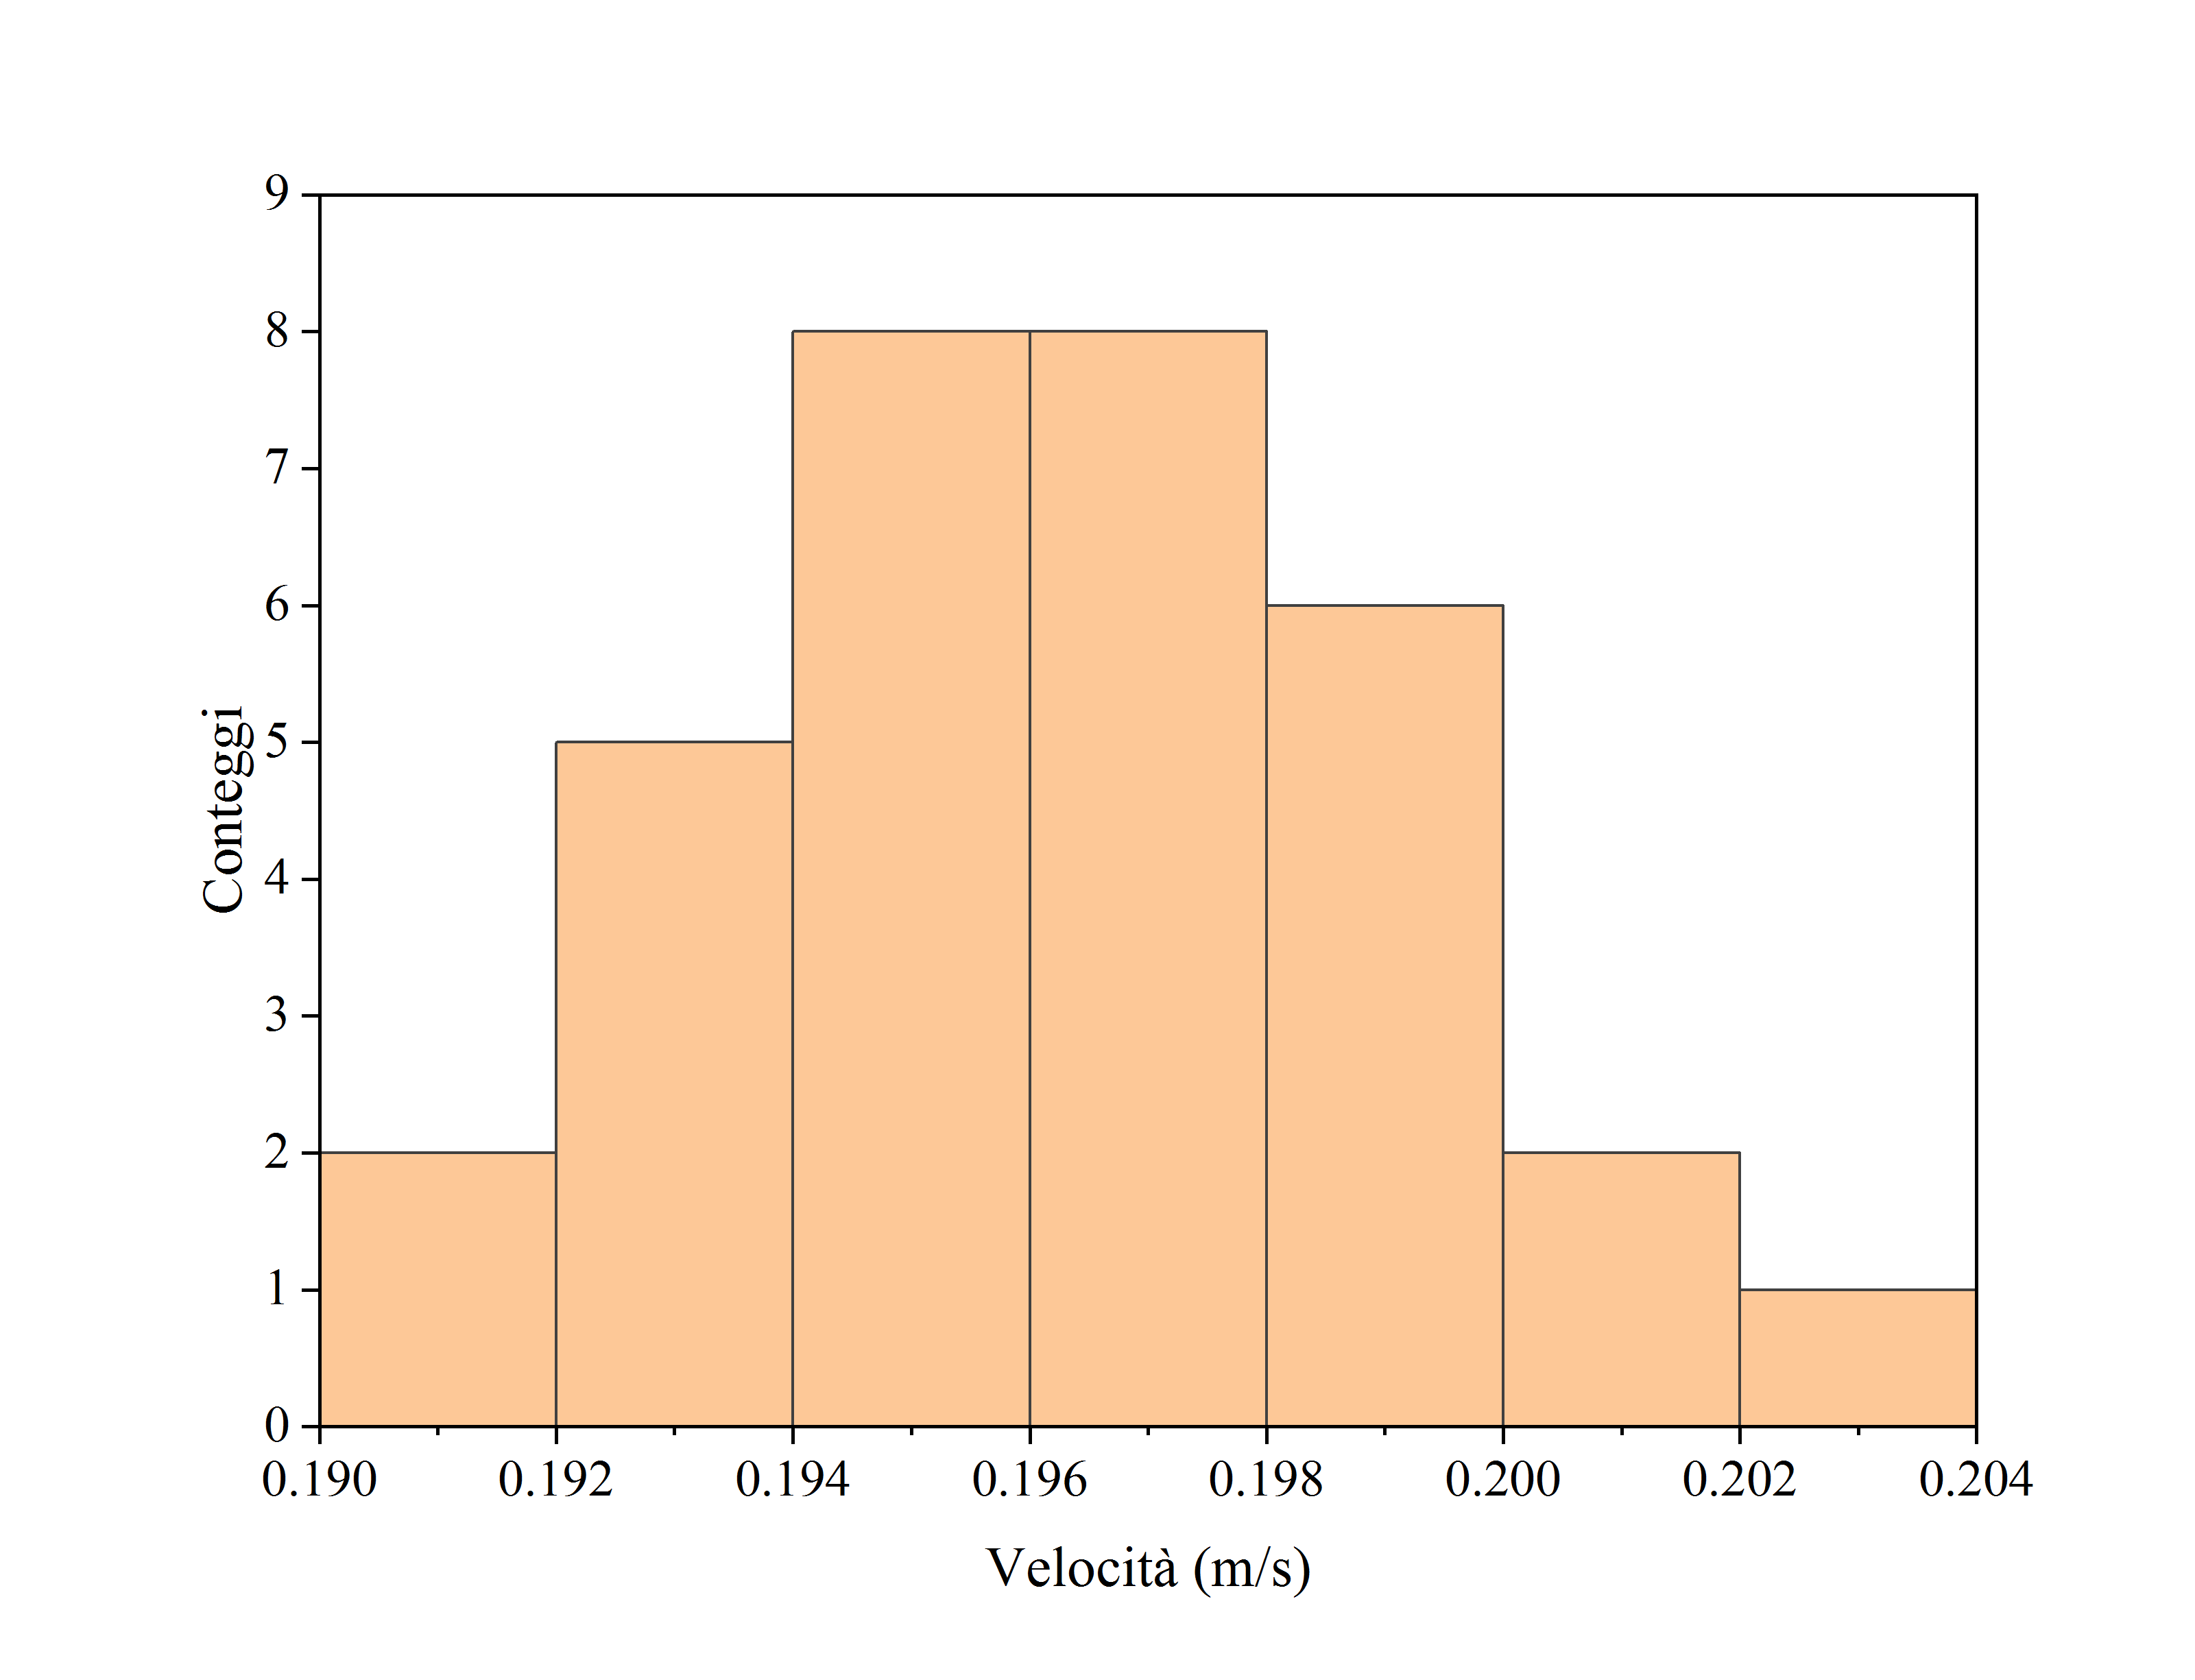
\includegraphics[trim={1cm 0.6cm 1cm 1cm},clip,width=.49\textwidth]{img/g1.png}}
    \hfil\subfloat[][
      Secondo giorno: Grandi ($N=28$)

      $\overline{v}=(14.48\pm0.06)\cdot10^{-2}\,\unit{m\per s}$
    ]{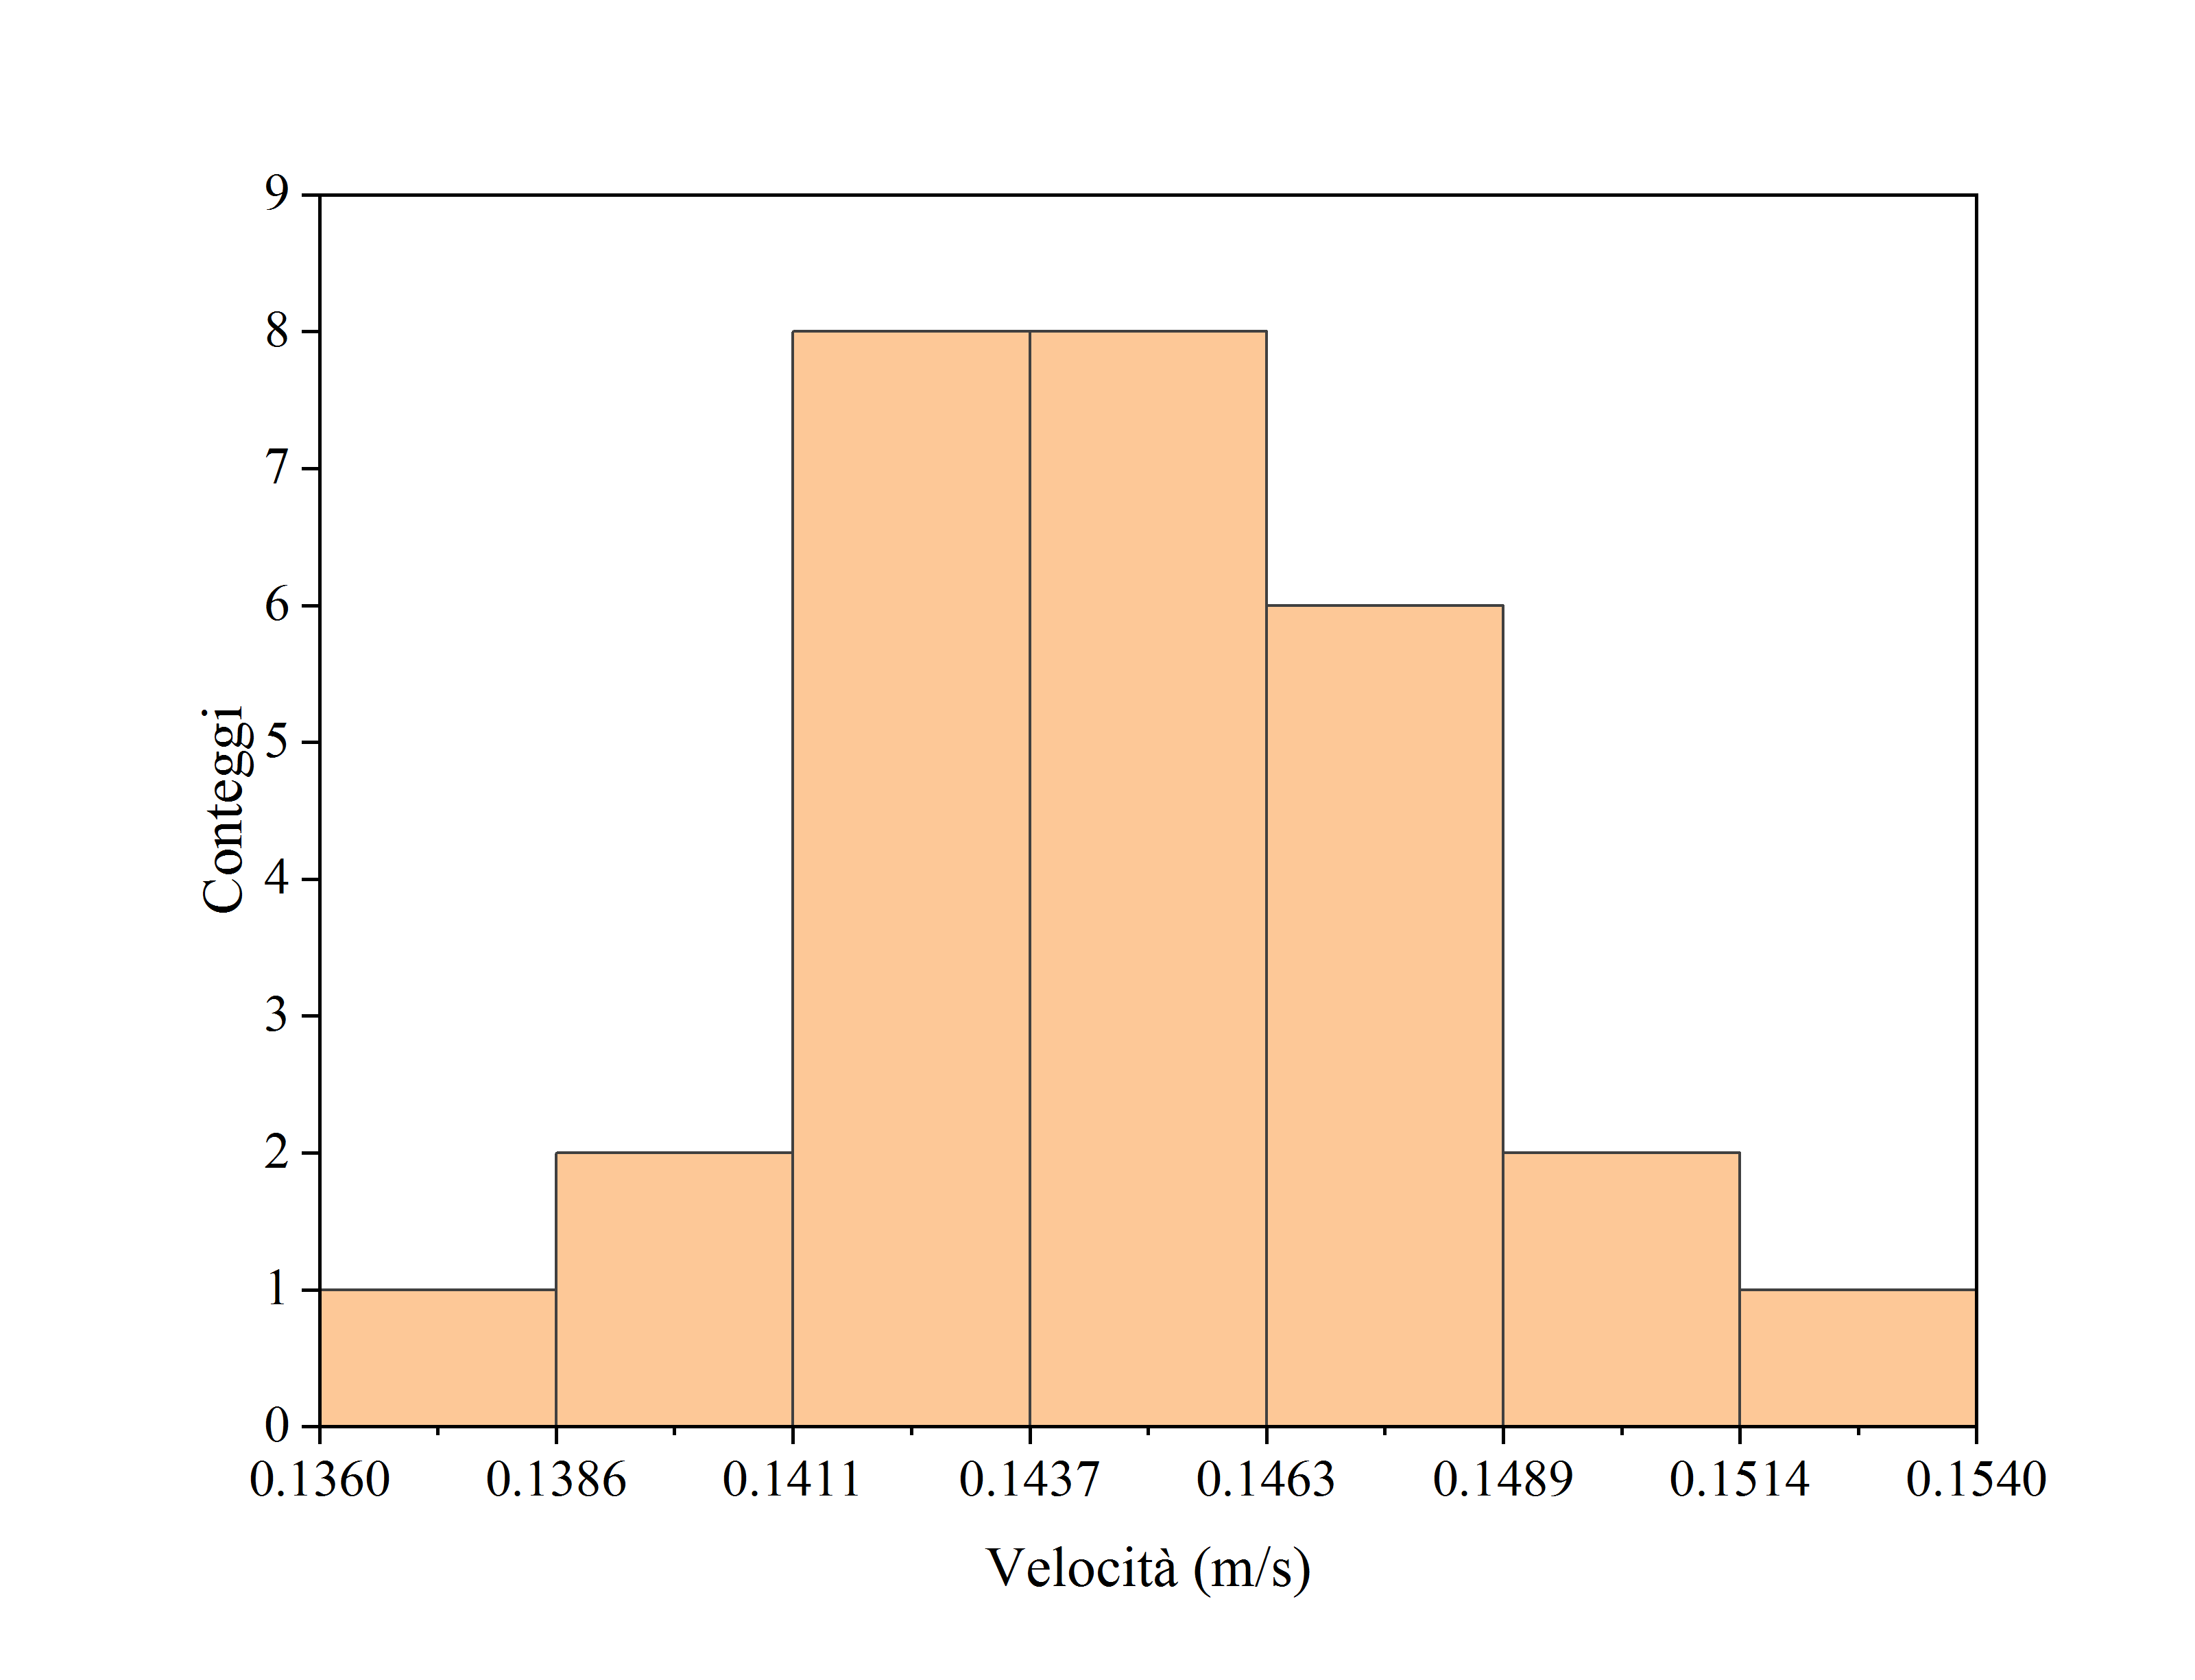
\includegraphics[trim={1cm 0.6cm 1cm 1cm},clip,width=.49\textwidth]{img/g2.png}}
  \end{figure}
\end{center}

\vspace{2mm}
\pagebreak
\emph{
  \textbf{Nota.} In questa sezione abbiamo trascurato la presenza di
  attriti, ma chiaramente gli attriti ci sono e il moto è smorzato.
  Nella sezione successiva tratteremo proprio questo fenomeno,
  determinando, alla luce dei dati raccolti, quanto influisca
  sul valore di $g$.
}
\vspace{2mm}

Poiché l'unica forza esterna al sistema che compie un momento lungo
$\hat{k}$ è la forza peso, si ha:
\[
  \sum\vec{\tau}^\text{\,ext}_z =
  \vec{r}_\text{CM}\times M\vec{g} = -Mg\,r_\text{CM}\sin(\theta)\hat{k}.
\]

L'equazione differenziale che descrive il moto del centro di massa
del pendolo fisico sarà allora:
\[ \ddot{\theta} = -\frac{Mg\,r_\text{CM}}{I_z^\text{tot}}\sin(\theta) \]

È possibile semplificare il modello fisico approssimando
$\sin(\theta)\simeq\theta$. Il gruppo di lavoro ha ritenuto
valida questa operazione solo quando
\[\left|\theta_0-\sin(\theta_0)\right| < \delta\theta\]

Essendo, nel nostro caso, $\delta\theta=\qty{0.02}{rad}$, abbiamo scelto
$\theta_0^\text{max} = \qty{0.49}{rad}$. Infatti:
\[
  \qty{0.49}{rad} - \sin(\qty{0.49}{rad}) \simeq \qty{0.019}{rad}
  \qquad
  \qty{0.50}{rad} - \sin(\qty{0.50}{rad}) \simeq \qty{0.021}{rad}
\]

Prima di prendere ogni misura, il gruppo di lavoro si è assicurato
che $\theta_0$ soddisfacesse abbondantemente la condizione
$|\theta_0|<\left|\theta_0^\text{max}\right|$.

L'equazione differenziale semplificata è allora:
\[ \ddot{\theta} = -\frac{Mg\,r_\text{CM}}{I_z^\text{tot}} \theta \]

Questa equazione descrive un moto armonico. Le soluzioni sono infatti
del tipo:
\[
  \theta(t) = \theta_0\cos(\omega t)
  \quad\text{dove}\quad
  \omega = \sqrt{\frac{Mg\,r_\text{CM}}{I_z^\text{tot}}}\quad\text{è detta “pulsazione”}.
\]

Possiamo tuttavia facilmente esprimere $\omega$ in funzione del periodo
$T$ del moto oscillatorio, più semplice da calcolare dai dati acquisiti.
Vale infatti:
\[
  \omega = \frac{2\pi}{T}
  \qquad\text{e quindi}\qquad
  \frac{I_z^\text{tot}}{Mr_\text{CM}} = g \frac{T^2}{4\pi^2}
\]

%\subsubsection{Il calcolo di $I_z^\text{tot}$ e $Mr_\text{CM}$}
La formula utilizzata per il calcolo di $I_z^\text{tot}$ riflette la composizione
del sistema, sfruttando la proprietà additiva del momento d'inerzia:
\[I_z^\text{tot} = I_{z,\text{rotore}} + I_{z,\text{asta}} + \sum_{\gamma\in\Gamma} I_{z,\gamma}\]

Chiaramente, per calcolare i momenti d'inerzia rispetto all'asse di
rotazione è necessario applicare il teorema di Huygens-Steiner
a quelli calcolati sui rispettivi centri di massa\footnote{
  Questi ultimi sono stati calcolati mediante le seguenti formule:
  \[
    I_\text{CM,asta} = \frac{1}{12} m_\text{asta} L_\text{asta}^2
    \qquad\quad
    I_{\text{CM},i} =
      \frac{1}{16}m_i\left(
        (d_i^\text{ext})^2 +
        (d_i^\text{int})^2
      \right) + \frac{1}{12} m_i h_i^2
    \quad\forall i \in \left\{A,B,C\right\}
  \]
}:
\[
  I_{z,\text{asta}} = I_\text{CM,asta} + m_\text{asta}\left(\frac{L_\text{asta} + \diam_\text{rotore}}{2}\right)^2
\]\[
  I_{z,(i,d)} = I_{\text{CM},i} + m_i\left(d + \frac{h_i - \diam_\text{rotore}}{2}\right)^2\qquad\forall(i,d)\in\Gamma
\]

Per calcolare il termine $M r_\text{CM}$, si osservi che, per la
definizione di posizione del centro di massa, la massa totale si
semplifica:
\[\begin{aligned}
  Mr_\text{CM} &= M\cdot \frac{1}{M}\left(
    m_\text{rotore}\cdot 0 + m_\text{asta} r_\text{CM,asta} +
    \sum_{(i,d)\in\Gamma}{m_i r_{\text{CM},i}}
  \right) \\&= m_\text{asta}\left(\frac{L_\text{asta} + \diam_\text{rotore}}{2}\right) +
    \sum_{(i,d)\in\Gamma}{m_i \left(d + \frac{h_i - \diam_\text{rotore}}{2}\right)}
\end{aligned}\]

Di seguito riportiamo le misure, dirette e indirette, utilizzate per il calcolo dei momenti d'inerzia\footnote{
  $L_\text{asta}$ è la lunghezza della parte dell'asta che sporge
  all'esterno del rotore.
}:

\begin{center}
  \begin{tblr}{ |c|c|c|c|c| }
    \hline
    Oggetto & $L\;\;(\unit{cm})$ & $\diam\;\;(\unit{mm})$ & $m\;\;(\unit{g})$ & $I_\text{CM}\;\;(10^{-5}\,\unit{kg\,m^2})$ \\
    \hline
    Asta & $60.0\pm0.1$ & $5.94\pm0.01$ & $45.82\pm0.01$ & $568.5\pm1.5$ \\
    \hline[dashed]
    Rotore & N./A. & $13.41\pm0.01$ & $22.4\pm0.1^*$ & $0.058\pm0.001^*$ \\
    \hline
  \end{tblr}
\end{center}\begin{center}
  \begin{tblr}{ |c|c|c|c|c|c| }
    \hline
    $i$ & $m_i\;\;(\unit{g})$ & $d_i^\text{\,ext}\;\;(\unit{mm})$ & $d_i^\text{\,int}\;\;(\unit{mm})$ & $h_i\;\;(\unit{mm})$ & $I_{\text{CM},i}\;(\unit{mg\,m^2})$ \\
    \hline
    A & $115.95\pm0.01$ & $29.95 \pm 0.05$ & $6.20 \pm 0.05$ & $19.93 \pm 0.01$ & $10.62\pm0.03$ \\
    \hline[dashed]
    B & $115.86\pm0.01$ & $29.95 \pm 0.05$ & $6.20 \pm 0.05$ & $19.89 \pm 0.01$ & $10.59\pm0.03$\\
    \hline[dashed]
    C & $71.46\pm0.01$ & $29.95 \pm 0.05$ & $6.20 \pm 0.05$ & $12.08 \pm 0.01$ & $5.047\pm0.018$\\
    \hline
  \end{tblr}
\end{center}

\emph{$[^*]$ Valori dati}

\pagebreak
%\subsubsection{La misura di $T$}
Il periodo dell'oscillazione è stato misurato individuando $N+1$ zeri
consecutivi di $\theta(t)$, diciamo $\left\{t_0,t_1,\dots,t_N\right\}$.
Allora, poiché tra uno zero e l'altro corre metà periodo, è possibile
calcolare $T$ in questo modo: $T = \frac{2}{N}(t_N - t_0)$

Il gruppo di lavoro ha scelto $N$ di volta in volta, in modo tale che
fosse proporzionale al numero di oscillazioni compiute dal pendolo
prima di fermarsi. Complessivamente, $N$ ha assunto valori da $30$ a
$180$.

\vspace{2mm}
%\subsubsection{Il calcolo di $g$}

Come descritto sopra, il gruppo di lavoro ha calcolato, per ogni
configurazione $\Gamma$,
i valori di $\frac{I_z^\text{tot}}{Mr_\text{CM}}$
e $\frac{T^2}{4\pi^2}$, riportati nel grafico seguente.

Come è possibile osservare dalla relazione che le lega, la dipendenza
tra queste due grandezze è lineare: questo ci permette di determinare
il valore di $g$ come coefficiente angolare di una retta di regressione.

\begin{center}
\begin{figure}[H]
  %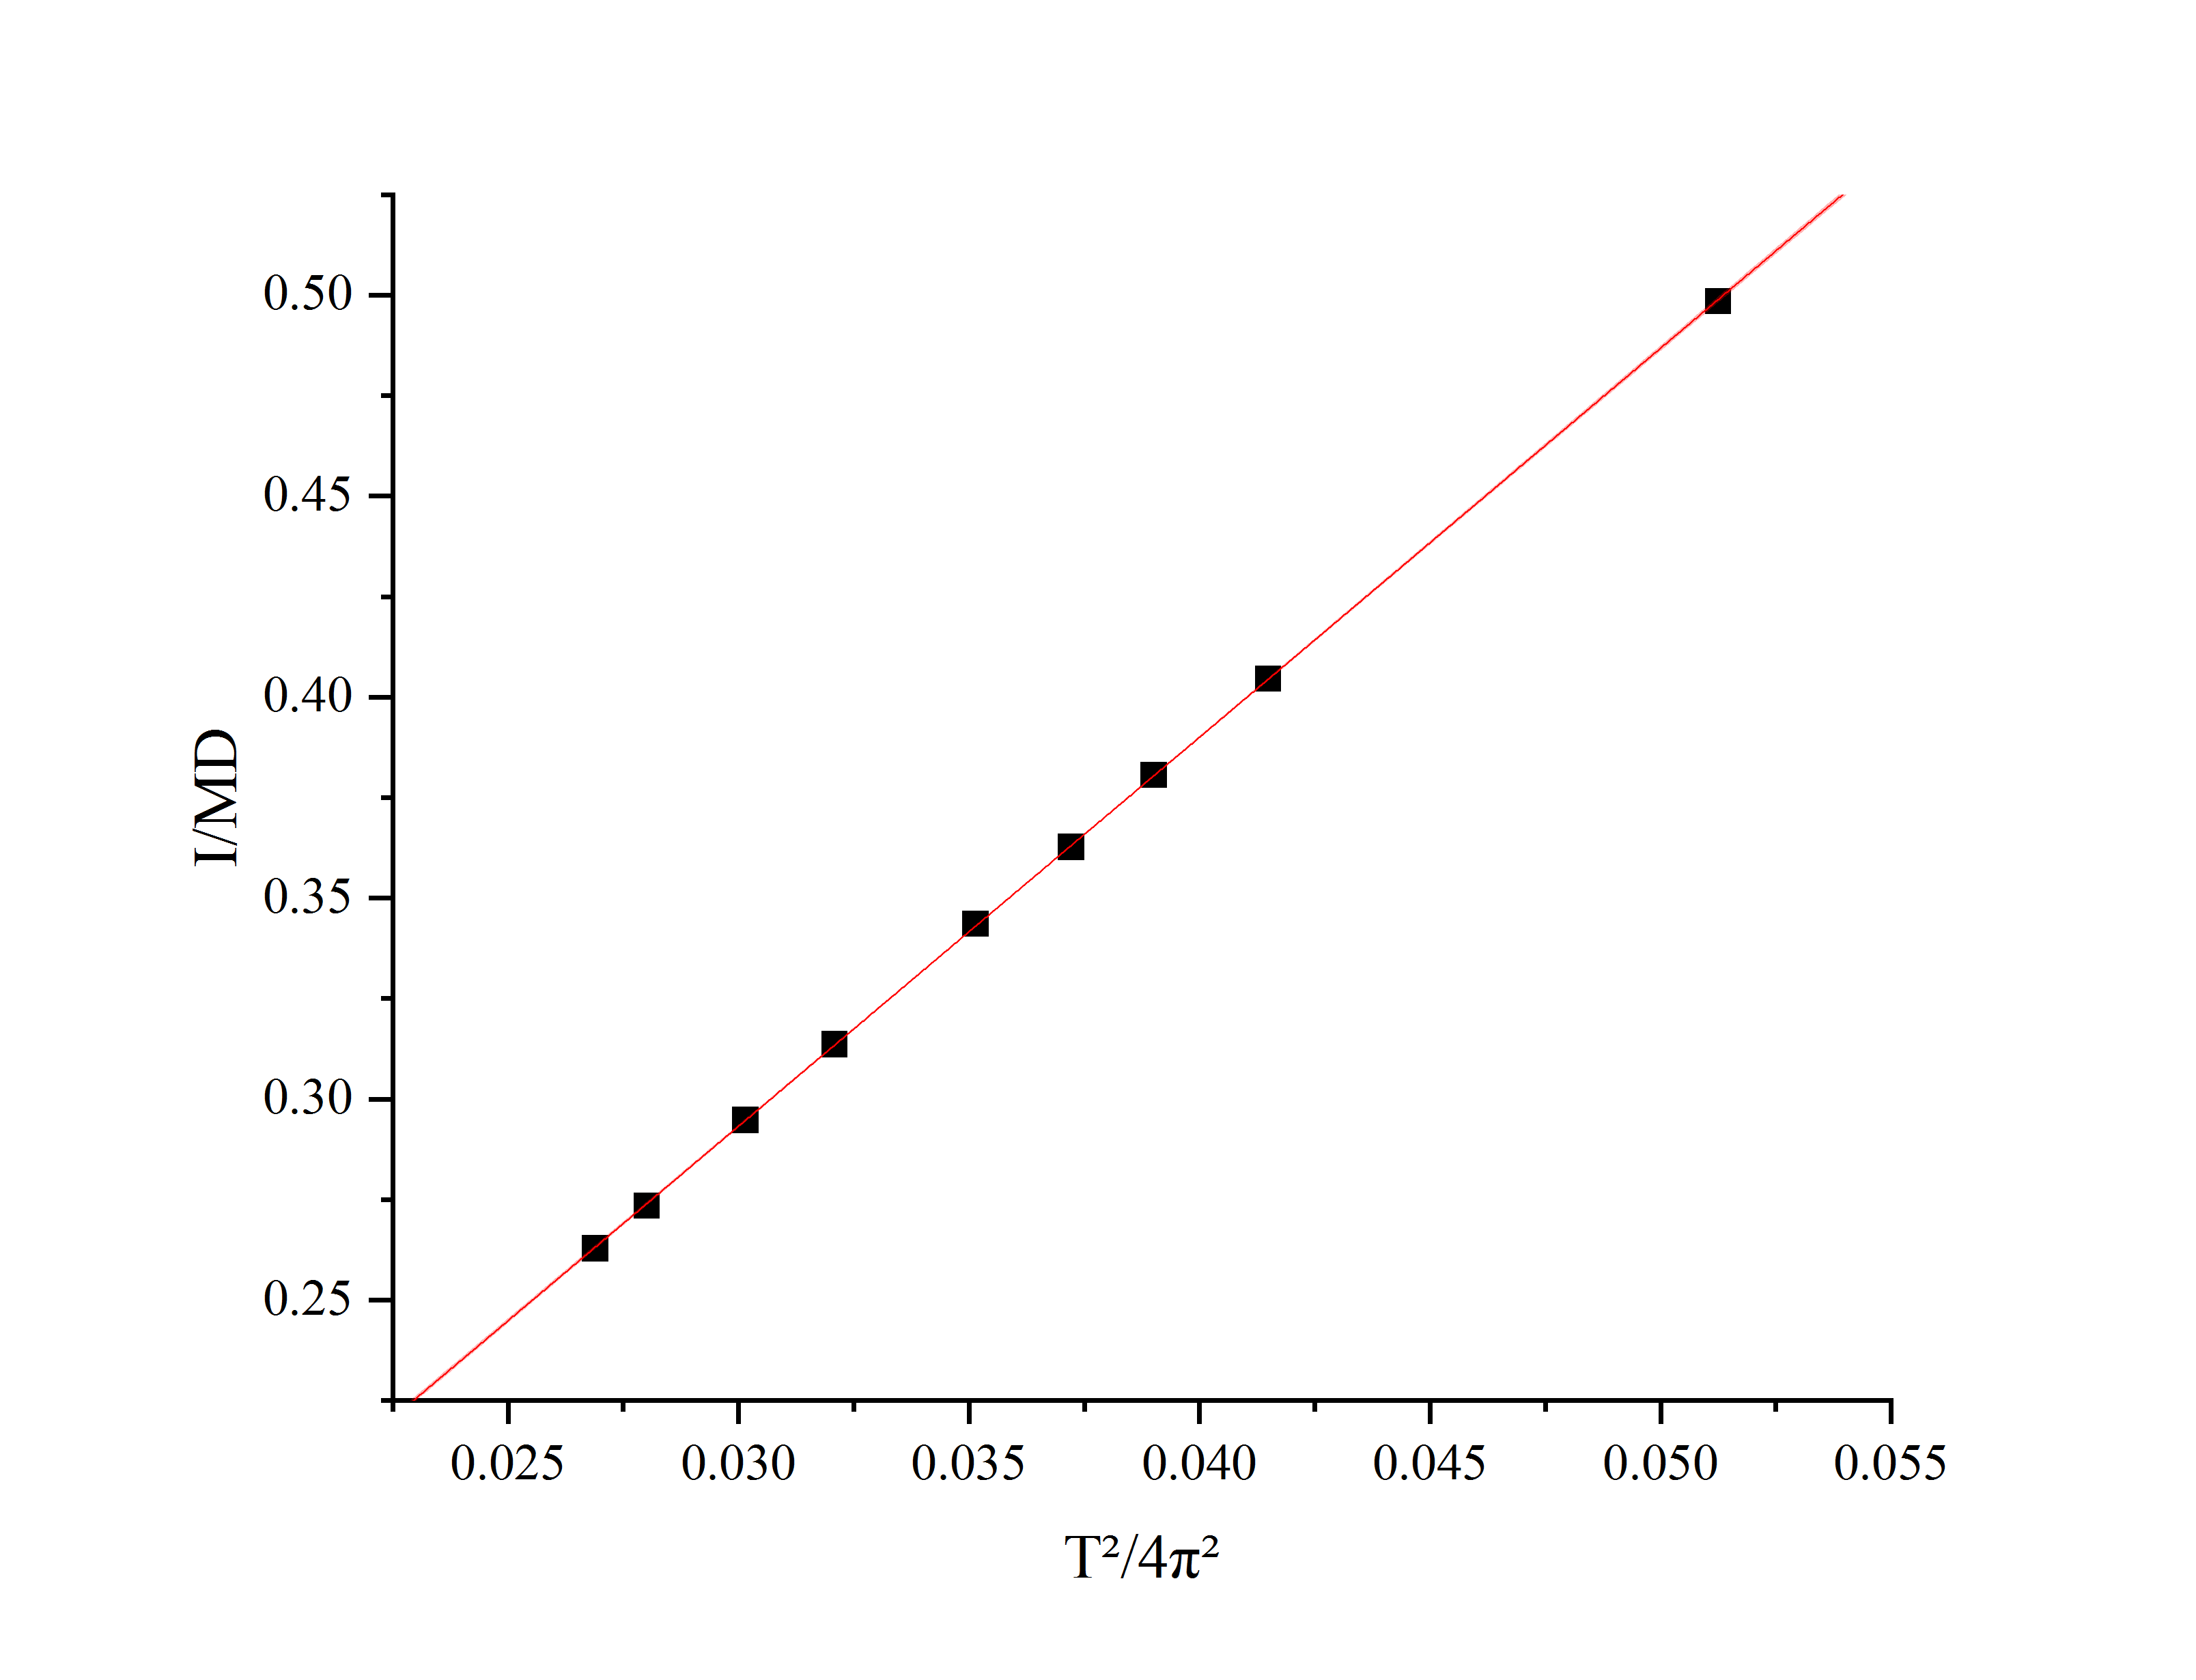
\includegraphics[trim={2cm 1cm 2cm 2.1cm},clip,width=\textwidth]{img/regressione.png}
  \caption[]{\emph{
    In rosso, la retta di regressione lineare e in rosa,
    appena visibile, la sua regione di incertezza.
    (le barre di errore sull'ascissa sono così ridotte
    da risultare invisibili)
  }}
\end{figure}
\end{center}

\begin{itemize}
  \item Intercetta $= (0.003 \pm 0.005)\;\unit{m}$
  \item Coefficiente angolare $g = (9.68 \pm 0.13)\;\unit{m\per s^2}$
\end{itemize}
\pagebreak
I risultati della regressione lineare sono chiaramente compatibili
con i valori attesi. Infatti:
\begin{itemize}
  \item Secondo il modello fisico utilizzato, l'intercetta dovrebbe
  essere nulla; in effetti, $(0.003\pm0.005)\;\unit{m}$ è compatibile
  con $\qty{0}{m}$.
  \item Il valore di $g$ atteso è $\qty{9.806}{m\per s^2}$; si può
  osservare facilmente che il valore misurato,
  $(9.68\pm0.13)\;\unit{m \per s^2}$, è compatibile con esso.
\end{itemize}

Possiamo pertanto concludere che l'esperienza ha avuto successo:
mediante l'apparato sperimentale abbiamo ottenuto una misura di $g$
compatibile con quella attesa.

\pagebreak
\subsection{Misura dello smorzamento}

\emph{
  In questa sezione, illustreremo come il gruppo di lavoro abbia
  valutato lo smorzamento del moto e quanto questo sia significativo,
  prendendo come esempio la configurazione $\Gamma=\left\{\right\}$,
  dove il pendolo fisico è composto solamente da asta e rotore, senza
  l'aggiunta di cilindri.
}

\emph{
  Il gruppo di lavoro ha effettuato gli stessi passaggi per tutte le
  altre configurazioni: i risultati saranno messi in evidenza alla
  fine della sezione.
}
\vspace{2mm}

Sempre applicando la seconda equazione cardinale della dinamica,
è facile ricavare l'equazione differenziale che caratterizza il moto
del sistema sotto l'effetto delle forze di attrito.
Approssimando, come prima, $\sin(\theta)\simeq\theta$, si ottiene:
\[ \ddot{\theta} = -2\lambda\dot{\theta} -\frac{Mg\,r_\text{CM}}{I_z^\text{\,tot}} \theta \]

dove $\lambda$ è una costante legata allo smorzamento del moto.
Le soluzioni di questa equazione differenziale sono infatti della forma:
\[\theta(t) = \theta_0\cos(\omega t)\,e^{-\lambda t}\]

dove la pulsazione del moto, $\omega$, è data da:
\[
  \omega^2 = \omega_0^2 - \lambda^2
  \qquad\text{con}\qquad
  \omega_0 = \sqrt{\frac{Mg\,r_\text{CM}}{I_z^\text{\,tot}}}.
\]

\begin{center}
  \begin{figure}[H]
    % trim={< v > ^}
    %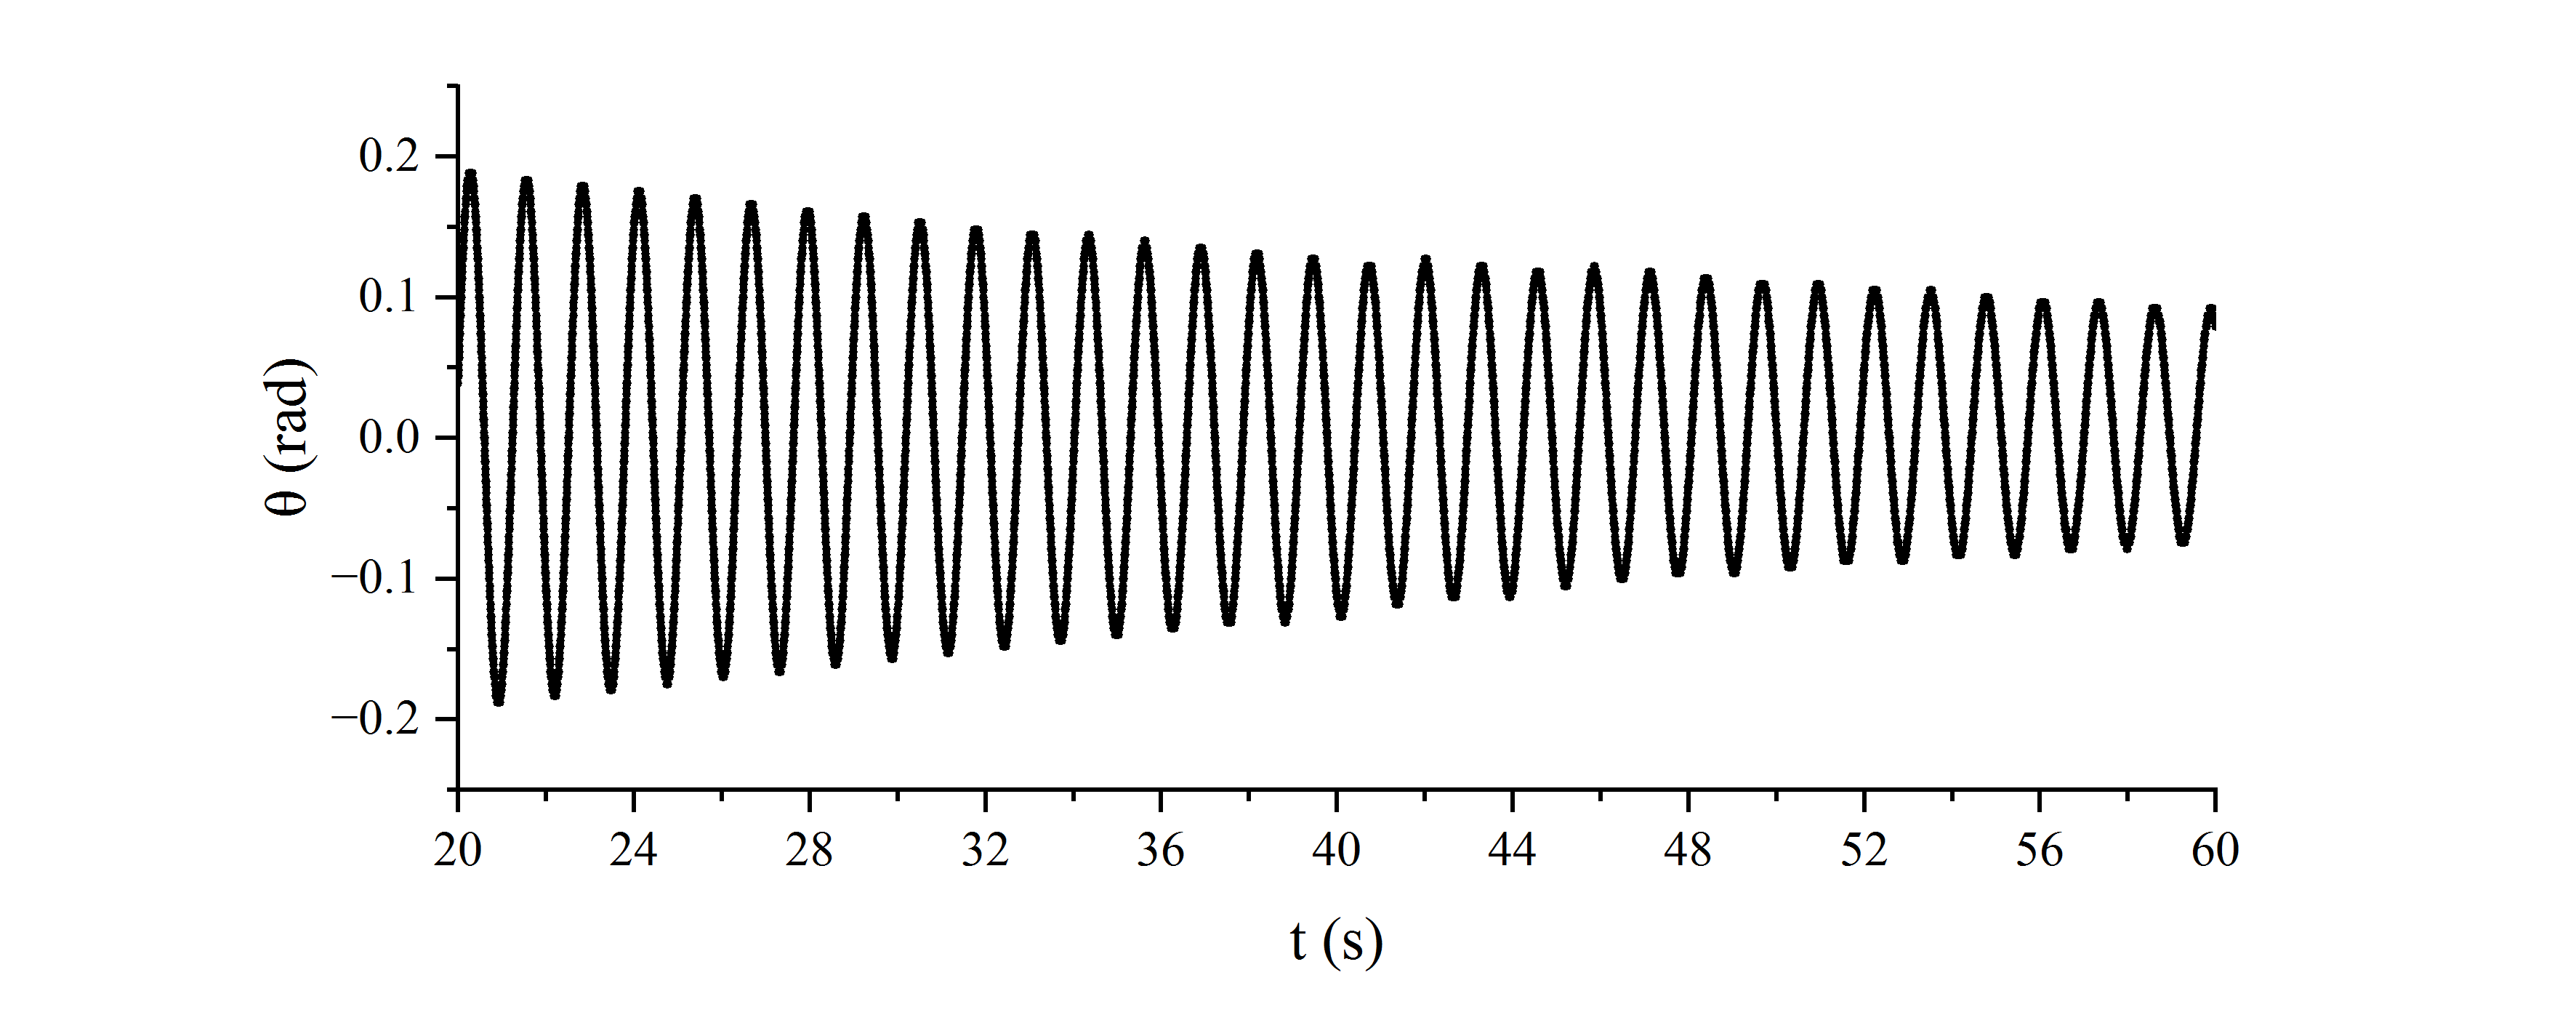
\includegraphics[trim={2cm .5cm 2cm .5cm},clip,width=\textwidth]{img/Graph1.png}
    \caption[]{\emph{
      Parte dei dati di un'acquisizione di $\theta(t)$
      con $\Gamma=\left\{\right\}$,
      come raccolti dal sensore di rotazione,
      riportati su una larga scala temporale.
      Si può chiaramente notare lo smorzamento
      del moto.
    }}
  \end{figure}
\end{center}

Per stimare $\lambda$, il gruppo di lavoro ha proceduto come segue:
\begin{enumerate}
  \item
    Per prima cosa, abbiamo individuato i massimi dei nostri dati,
    ovvero gli insiemi di punti della forma
    $\left\{t_i,t_{i+1},\dots,t_j\right\}\times\left\{\theta_k\right\}$
    tali che $\theta(t_{i-1}) < \theta_k > \theta(t_{j+1})$.
  \item
    Per ogni massimo, ne abbiamo calcolato il punto medio,
    prendendo come $\delta t_\text{picco}$ la semidispersione $\frac{1}{2}(t_j - t_i) + \delta t$.
  \item
    Infine, abbiamo graficato i punti così trovati
    su scala logaritmica e
    abbiamo effettuato una regressione lineare (pesata\footnote{
      $\delta\!\ln{\left|\theta\right|}$, infatti, varia molto,
      nonostante $\delta\!\left|\theta\right|$ sia costante:
      ciò è conseguenza della propagazione degli errori.
      È inoltre possibile osservarlo nella \emph{Figura 2}.
    })
    sulle nuove ordinate. Il coefficiente angolare di tale
    regressione dovrebbe essere proprio $-\lambda$.
  \item
    Abbiamo ripetuto i tre punti precedenti sugli stessi dati,
    con $\theta$ cambiato di segno: così facendo, ai massimi
    si sostituiscono i minimi e tutto il resto dell'analisi
    è analoga. Per ogni configurazione abbiamo pertanto ottenuto
    due diversi valori di $\lambda$: $\lambda_\text{min}$ e
    $\lambda_\text{max}$. Abbiamo scelto di porre
    $\lambda=\frac{1}{2}(\lambda_\text{min}+\lambda_\text{max})$.
\end{enumerate}

\begin{center}
  \begin{figure}[H]
    % trim={< v > ^}
    %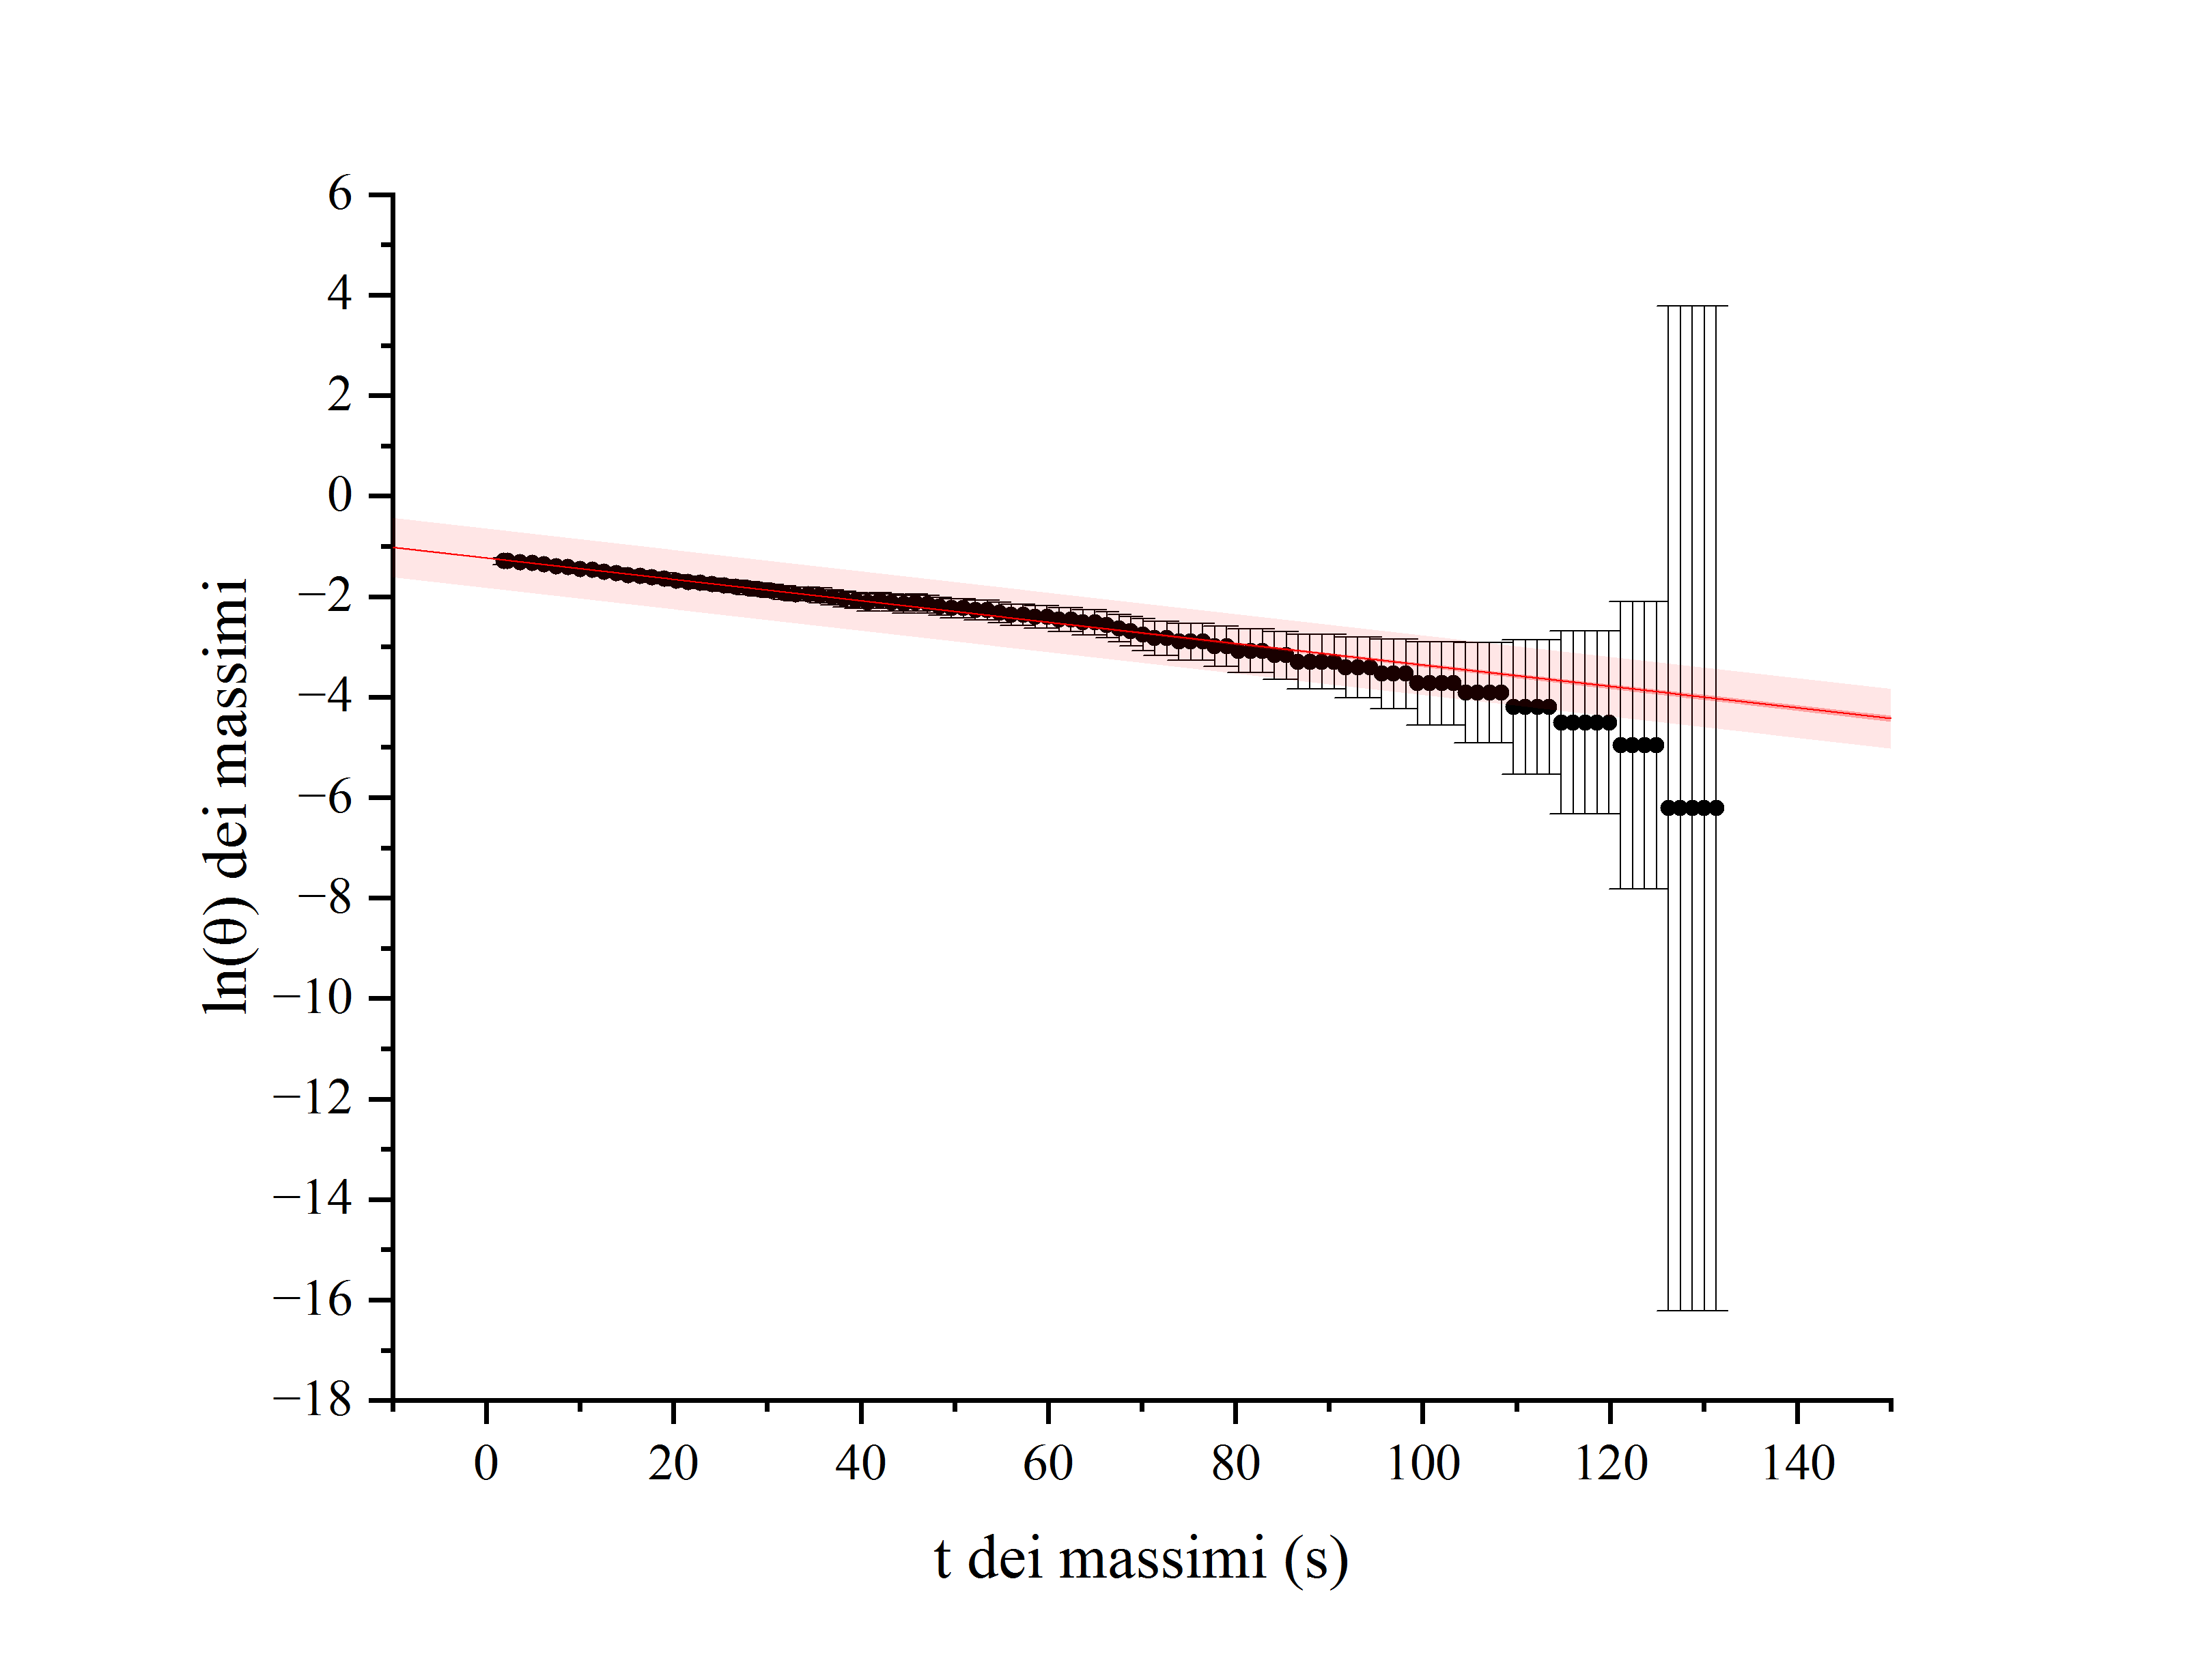
\includegraphics[trim={2cm 1cm 2cm 2.1cm},clip,width=.5\textwidth]{img/0max-exp.png}
    %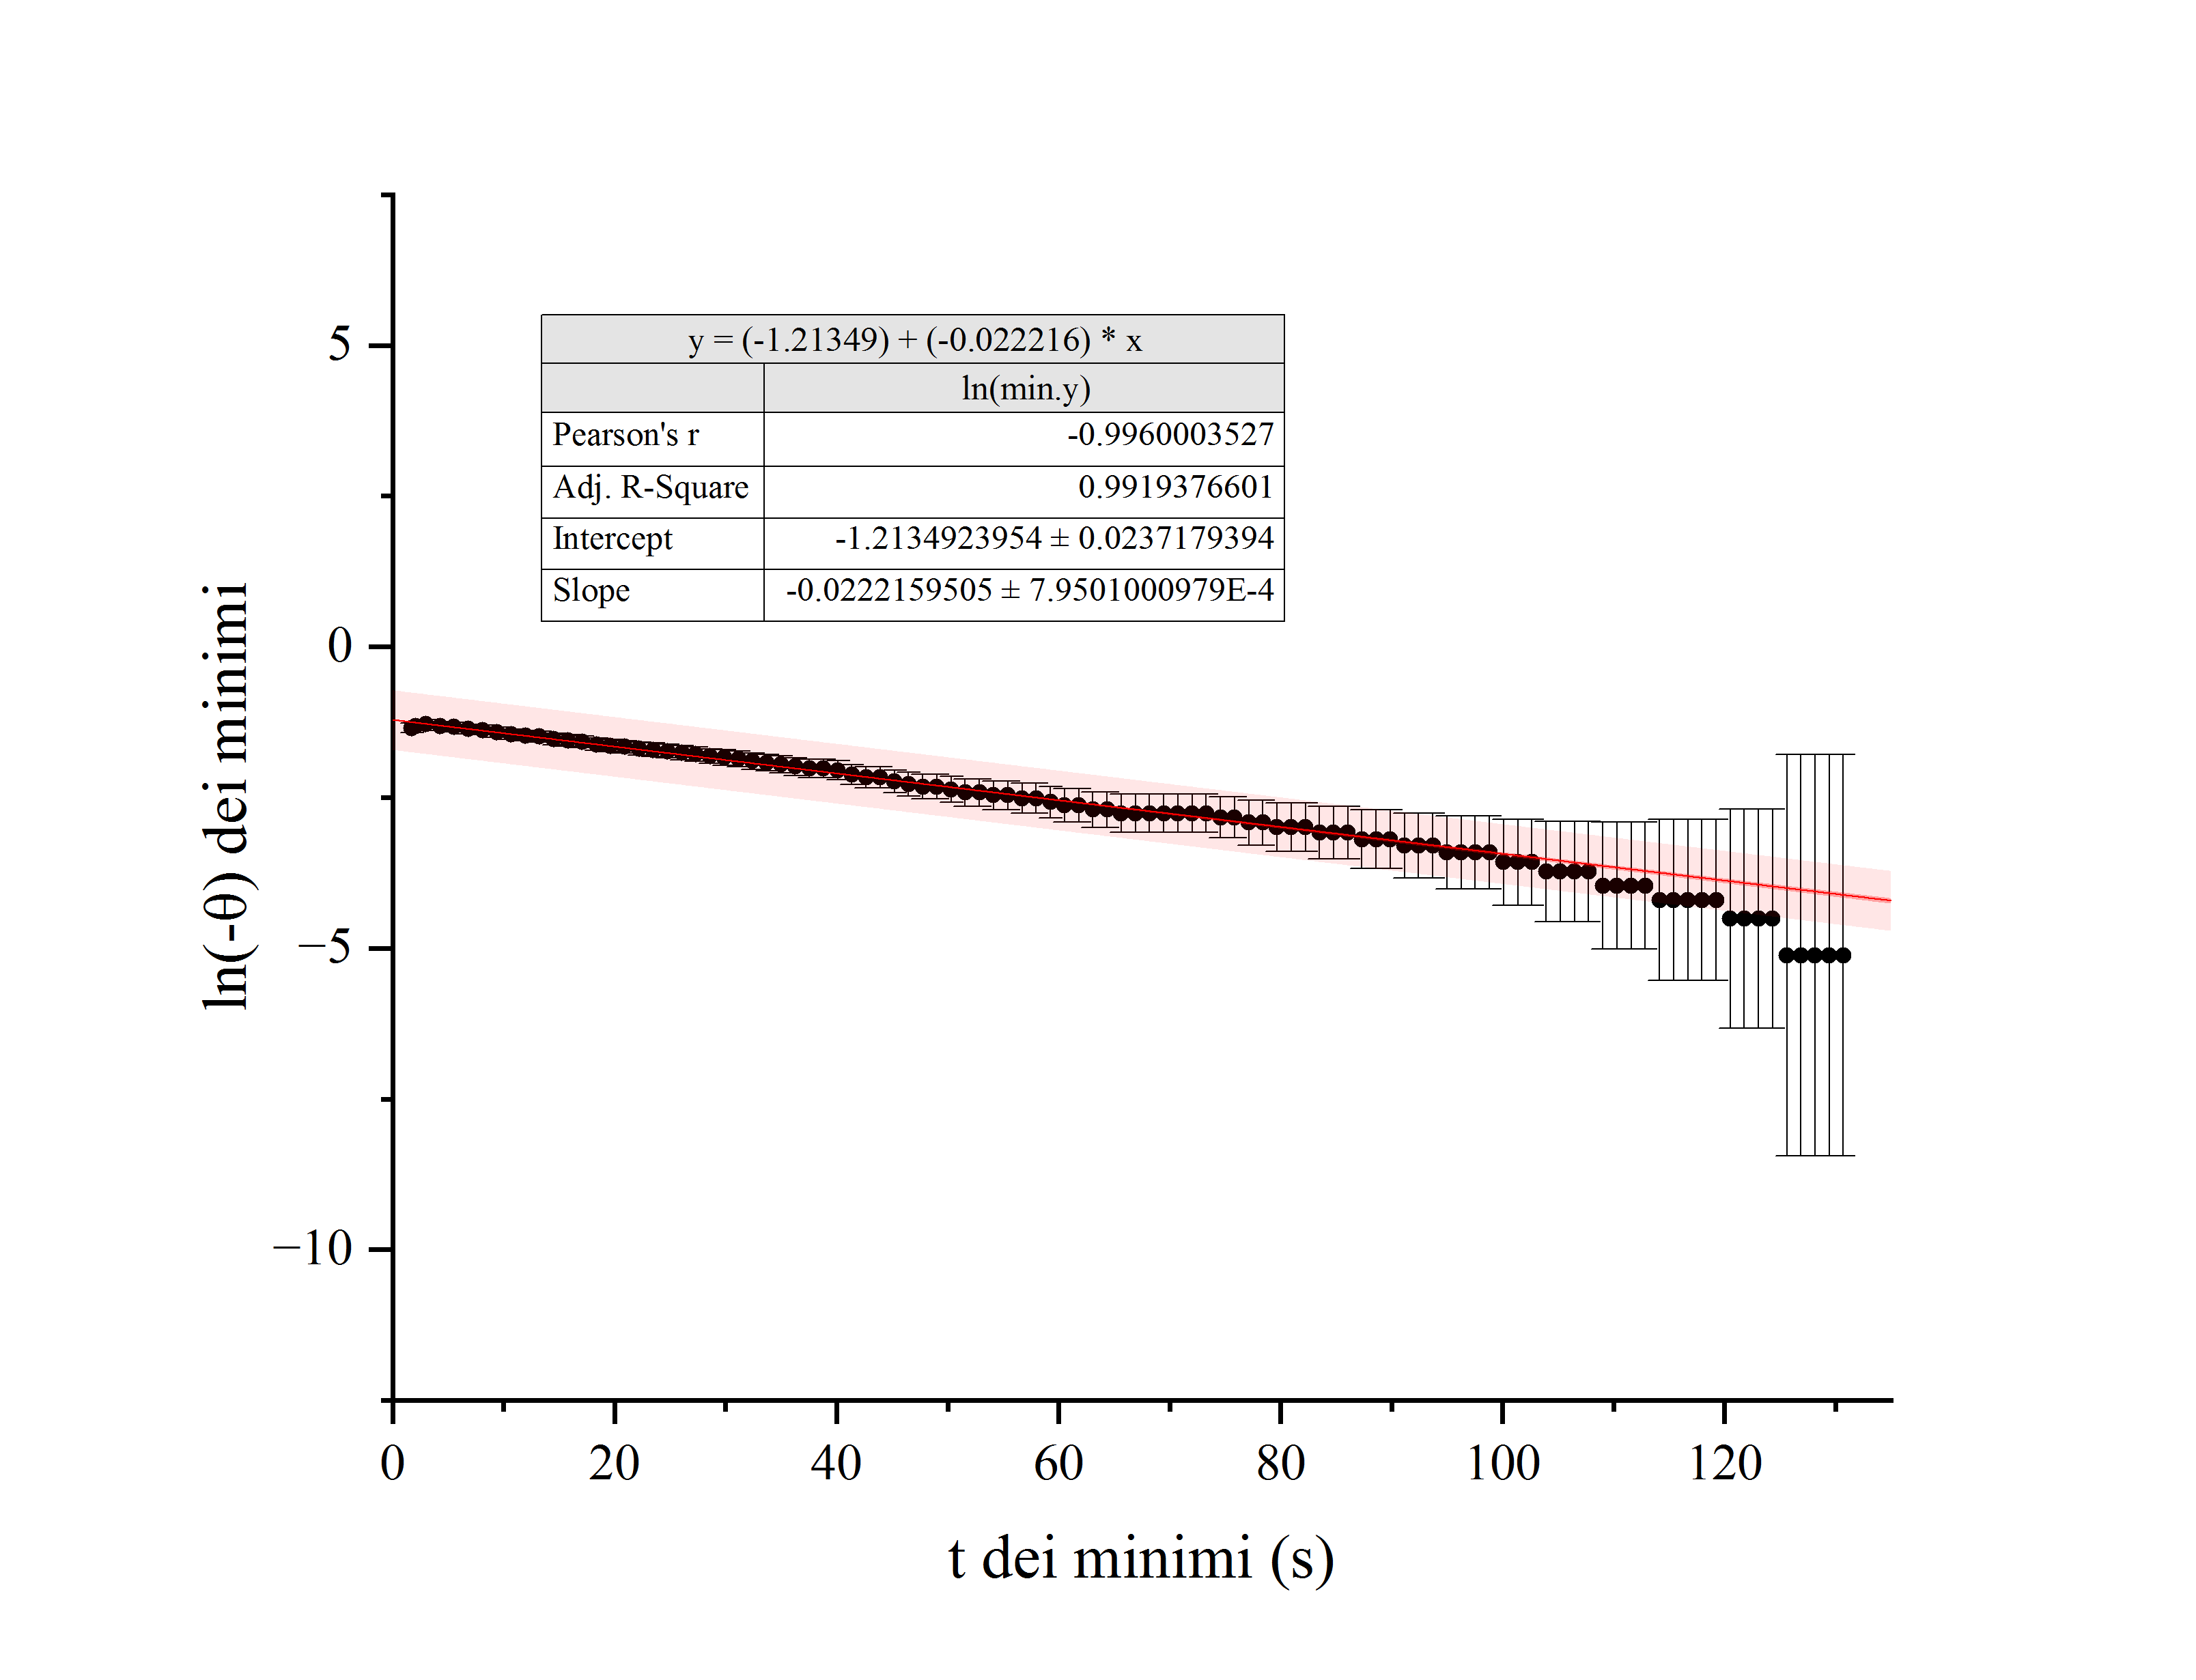
\includegraphics[trim={2cm 1cm 2cm 2.1cm},clip,width=.5\textwidth]{img/0min-exp.png}
    \caption[]{\emph{
      $\ln\left|\theta(t)\right|$ di massimi e minimi,
      su scala logaritmica (per $\Gamma=\left\{\right\}$).
      Sono riportate anche le barre di errore sull'ordinata.
      In rosso, la retta di regressione lineare
      e in rosa la sua regione di incertezza.
    }}
  \end{figure}
\end{center}

Poiché l'obiettivo è calcolare $g$, la correzione da effettuare
sul periodo, per tenere conto dell'attrito, è la seguente:
\[
  T_0^2 = \frac{4\pi^2}{\omega_0^2}
    = \frac{4\pi^2}{\omega^2 + \lambda^2}
    = \frac{4\pi^2}{\frac{4\pi^2}{T^2} + \lambda^2}
    = \frac{1}{\frac{1}{T^2} + \frac{\lambda^2}{4\pi^2}}
\]

Effettuata questa correzione per ogni configurazione $\Gamma$,
si può allora costruire nuovamente una retta di regressione,
analogamente a quanto fatto nella sezione precedente.
La relazione fra le grandezze misurate, ricordiamo, è lineare:
\[ \frac{I_z^\text{\,tot}}{Mr_\text{CM}} = g \frac{T_0^2}{4\pi^2} \]

Riportiamo di seguito il grafico della nuova regressione,
unitamente ai risultati ottenuti.

\begin{figure}[H]
  %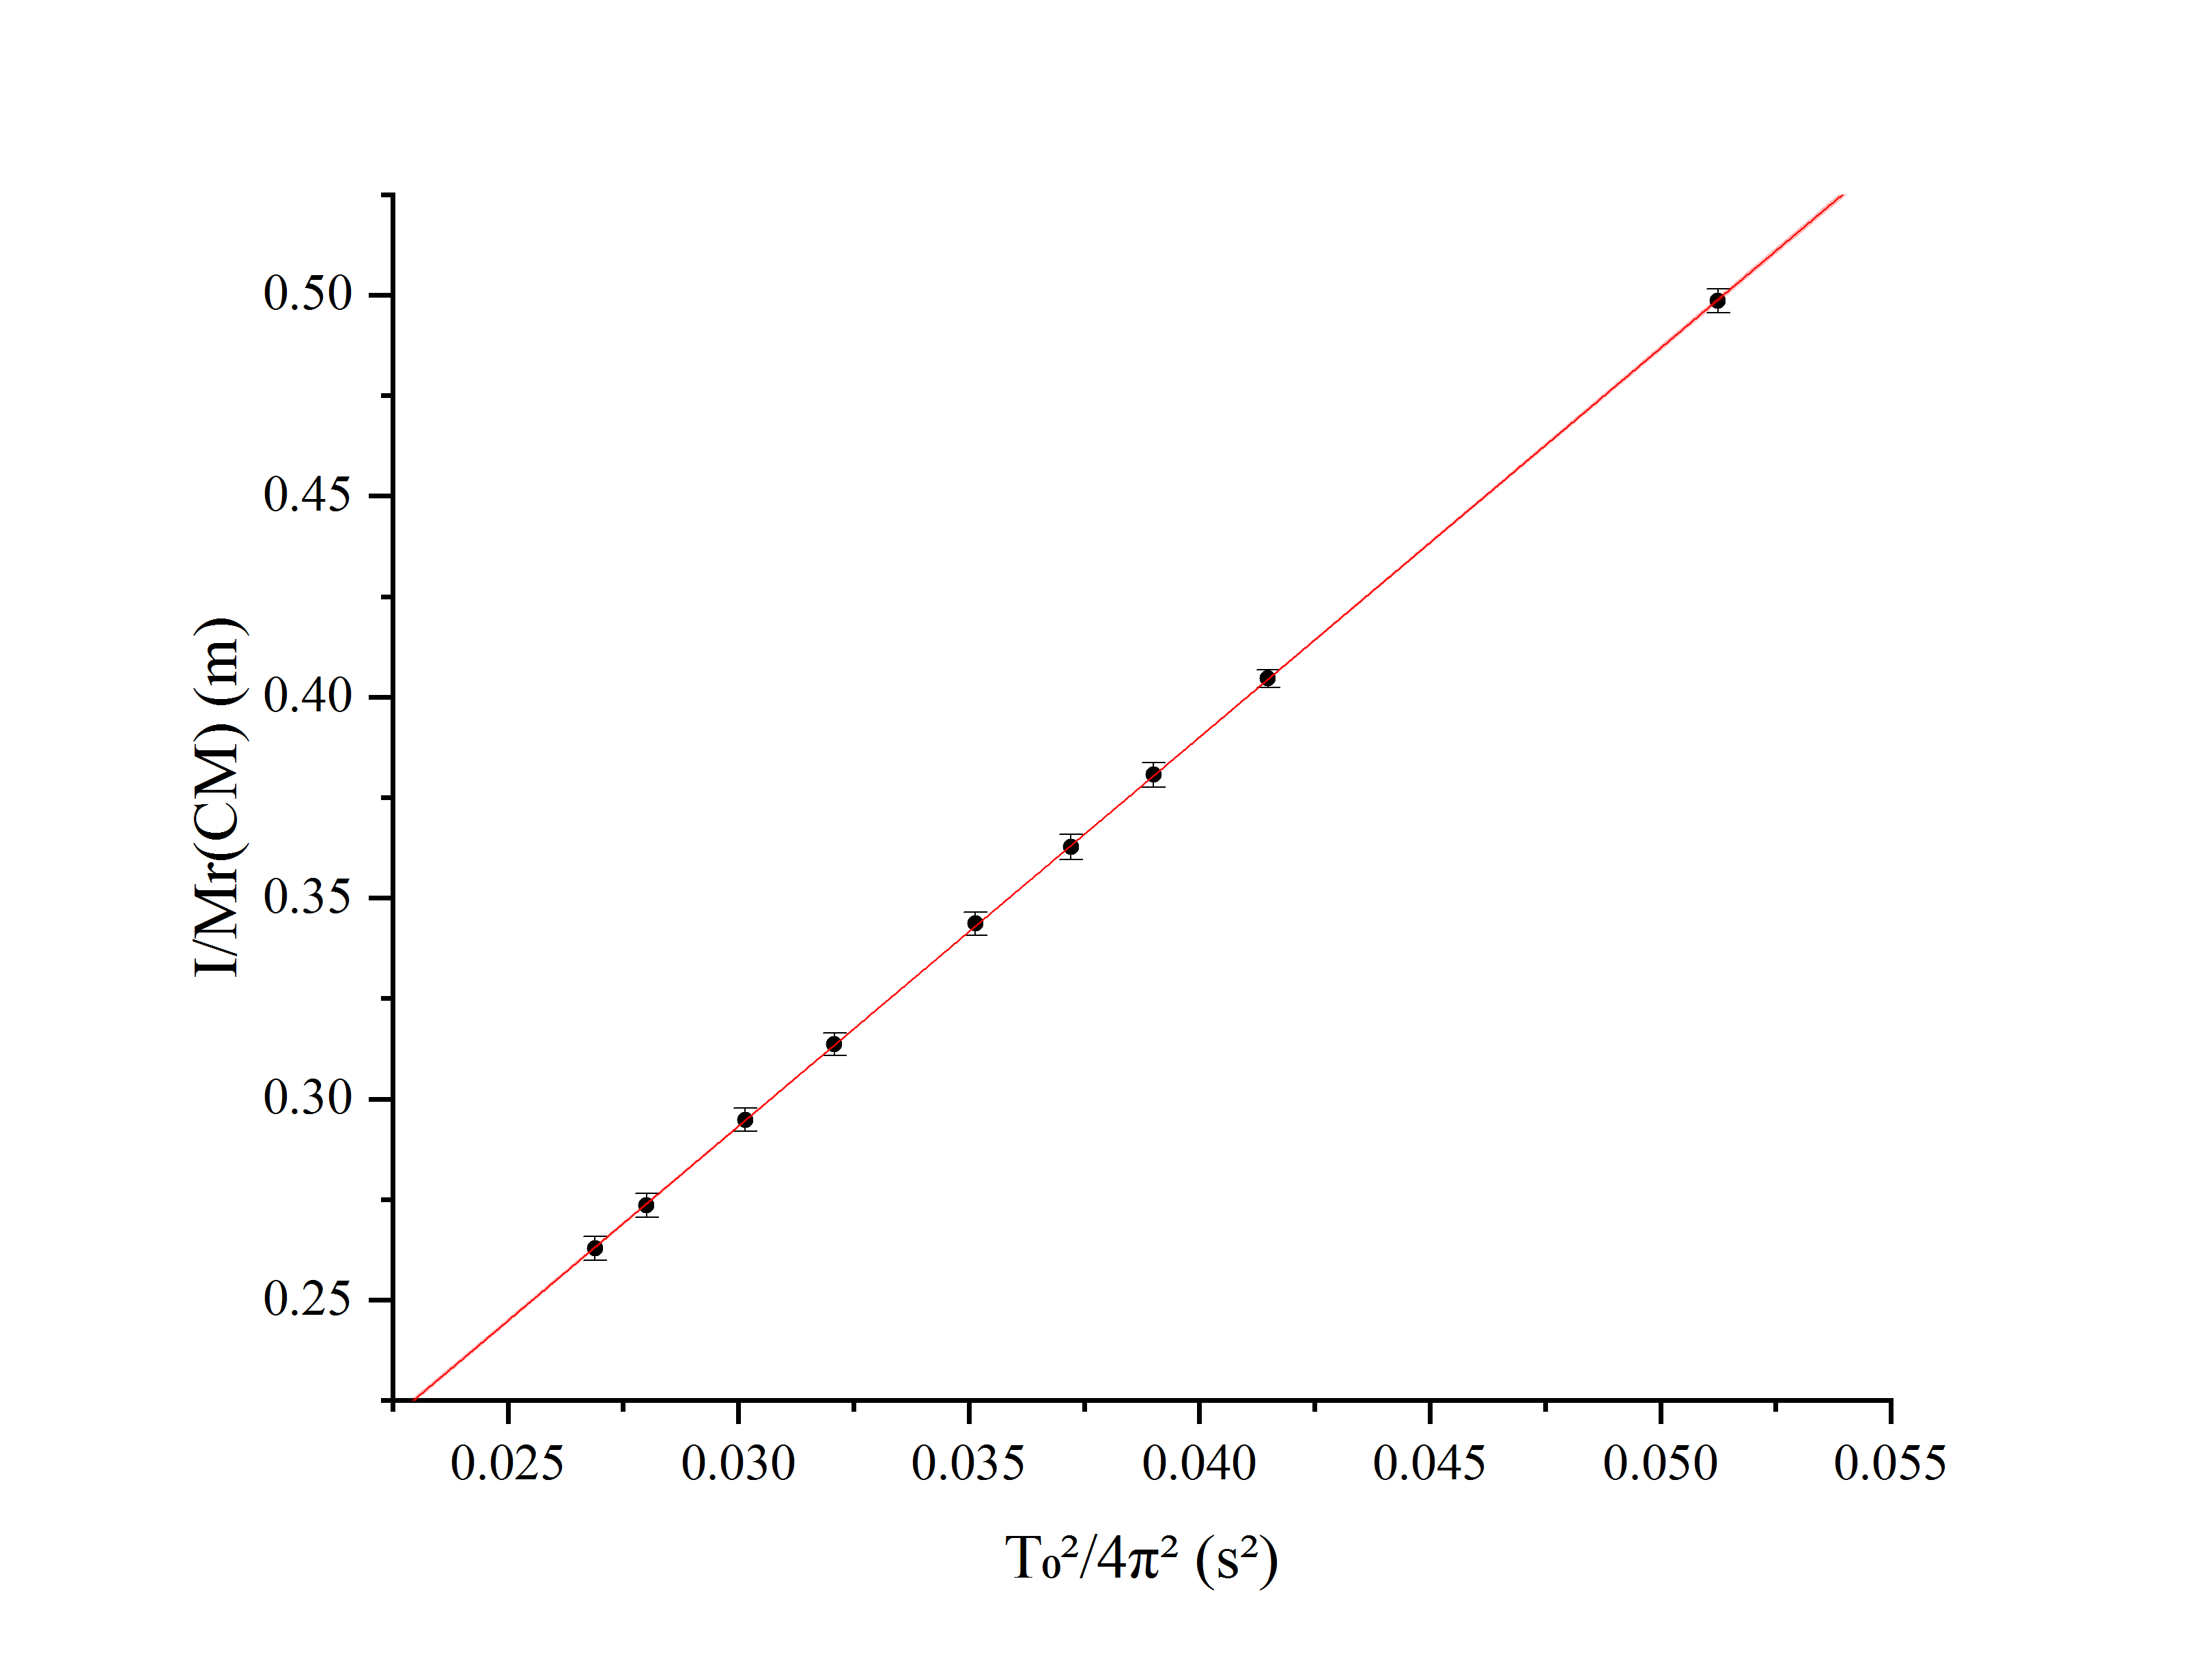
\includegraphics[trim={2cm 1cm 2cm 2.1cm},clip,width=\textwidth]{img/regressione-2.png}
  \caption[]{\emph{
    In rosso, la retta di regressione lineare e in rosa,
    appena visibile, la sua regione di incertezza.
    (le barre di errore sull'ascissa sono così ridotte
    da risultare invisibili)
  }}
\end{figure}

I risultati della regressione lineare sono i seguenti:
\begin{itemize}
  \item Intercetta $= (0.003 \pm 0.005)\;\unit{m}$
  \item Coefficiente angolare $g = (9.68 \pm 0.13)\;\unit{m\per s^2}$
\end{itemize}

Come è possibile osservare comparando questi risultati a
quelli precedentemente ottenuti, il valore di $g$ risultante
è rimasto essenzialmente invariato (al netto della sua incertezza).

In conclusione, possiamo affermare ragionevolmente che,
rispetto alla sensibilità degli strumenti di misura,
il contributo dell'attrito è trascurabile.

\end{document}
